\chapter{Methods} \label{sec: methods}

In this section we are going to present the proposed solutions. We have implemented an existing solution: Online LSTM Planner (replica of \cite{nicola2018lstm}) and developed three proposed solutions: CAE Online LSTM Planner, LSTM Bagging Planner and Global Way-point LSTM Planner. For each solution, we are going to theoretically prove the worst case (average case) space and time complexity, state the optimality conditions, state a few advantages and disadvantages and showcase a few algorithm runs on the synthetically generated maps (i.e. the training datasets). It should be noted that the detailed training information and exhaustive experiments will be presented in Chapter \ref {Evaluation} (\hyperref[Evaluation]{Evaluation}). % follow same convention

\textbf{Online LSTM Planner.} The planner attempts to replicate the solution from \cite{nicola2018lstm}. The algorithm essentially uses an LSTM network to retrieve the next action that the agent should take given the current location data (localisation and local surroundings information). The planner will be later used in the final proposed solution and provides a strong frame of reference for the empirical experiments.

\textbf{CAE Online LSTM Planner.} The algorithm is a hybrid solution between \cite{nicola2018lstm} and \cite{inoue2019robot} which attempts to fix some issues that are present in the Online LSTM Planner (e.g. the algorithm does not know how to navigate between complex obstacles and long corridors). This is done by augmenting the input from the LSTM network with the compressed global image snapshot (when we are dealing with partial knowledge environments, we are still going to use the global image snapshot, but we are going to include the unknown environment as well). The global snapshot is compressed using a Convolutional Auto-encoder (CAE).

\textbf{LSTM Bagging Planner.} It is a solution inspired by ML ensemble methods which combines the previous algorithms (Online LSTM Planner and CAE Online LSTM Planner) into a unique best-of-all kind of algorithm. The planner attempts to boost the performance of the previous algorithms by picking the best solution depending on the layout of the environment.

\textbf{Global Way-point LSTM Planner.} It represents the final proposed solution. The planner uses one local kernel and one global kernel. The global kernel is responsible for suggesting a series of way-points which will guide the agent through the environment and the local kernel is responsible for the actual manoeuvring between way-points. The planner uses the LSTM Bagging Planner as the global kernel by transforming it into a way-point suggestion algorithm. This is achieved by bounding the number of iterations of the LSTM Bagging Planner. Any classic solution can be used as the local planner, but we have decided to use A* as it represents the base algorithmic frame of reference against all other proposed solutions in Chapter \ref {Evaluation} (\hyperref[Evaluation]{Evaluation}).

\pagebreak

\section{Online LSTM Planner}

% The Online LSTM Planner
The Online LSTM Planner algorithm is a close replica of \cite{nicola2018lstm}, with some architectural and logic changes. The planner uses an LSTM network to query the next agent action (next movement) at each time step.

\subsection{LSTM Architecture}

The LSTM architecture takes four types of inputs: the normalised distance between the agent to obstacles on all eight directions (raycast\_8\_normalised(50)), the normalised direction to the goal (direction\_to\_goal\_normalised), the angle defined by the direction to the goal (agent\_goal\_angle) (not required to be normalised as it is already bounded by definition), the normalised distance to the goal (distance\_to\_goal\_normalised(100)) (See Figure \ref{fig:lstm_input_viz}) and returns the next agent action/movement index (next\_position\_index) (See Table \ref{tab: gen_label_list} for reference). No data pre-processing is done as the input is already normalised and we use batch normalisation layers. 

\begin{figure}[h!]
    \centering
    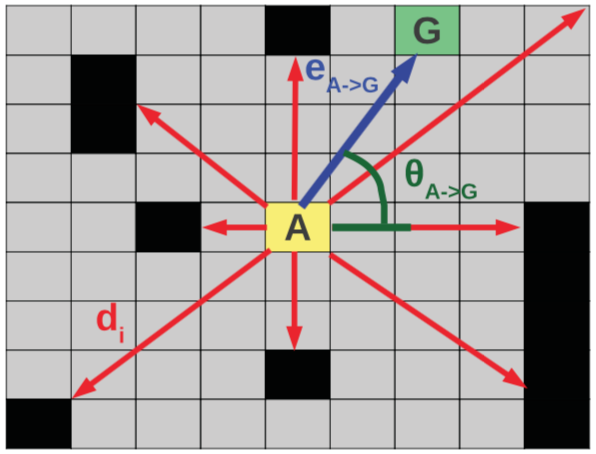
\includegraphics[scale=0.50]{images/paper_input.png}
    \caption{Input visualisation \cite{nicola2018lstm}. $d_{i}$ is raycast\_8\_normalised(50), $\theta_{A\xrightarrow{}G}$ is agent\_goal\_angle and $e_{A\xrightarrow{}G}$ is both direction\_to\_goal\_normalised and distance\_to\_goal\_normalised(100)}
    \label{fig:lstm_input_viz}
\end{figure}

The network uses the cross entropy loss function which combines both log softmax and negative log likelihood into a single function:
\begin{align*}
    L(\boldsymbol{x}, y) = - \log \frac{e^{x_y}}{\sum_j e^{x_j}} \textrm{, where \boldsymbol{x} is the prediction for all classes and y is the actual class}
\end{align*}
The model contains a hidden state and cell state which are initialised at each new batch with a 0 tensor of size $2 \times lstm\_layers \times batch\_size \times lstm\_output\_size$. The architecture has the following structure: one batch normalisation layer, two LSTM layers, one batch normalisation layer and one linear layer (See Figure \ref{fig:lstm_kernel}). 

The architecture of the network is almost identical to the one from \cite{nicola2018lstm}, but we do not feed the previous agent action as the paper does due to performance reasons. The data has to be constantly packed and unpacked before it is fed through the LSTM layers. When the data has to be passed through an LSTM layer, it is packed, and when it has to be passed through a linear layer, it has to be unpacked. If the previous action was added as an input, then the data had to be packed and unpacked for each sequence step from the batch, which is a severe performance downgrade (packing and unpacking is thoroughly described in Appendix \ref{sec: app_methods}). Moreover, because we use an LSTM network, the previous action information lies into the hidden and cell state already.

\textbf{Batch Normalisation Layer.} Unlike the paper, we use batch normalisation layers to speed up the learning process by reducing the covariance shift (the hidden unit values shift). Moreover, the network can generalise better for unseen examples if they belong to the same distribution as the training data (e.g. if we train the model on a dataset composed of black cats, the network will not identify coloured cats, but if we use batch normalisation, since coloured cats belong to the same distribution as black cats (both of them are cats and share the same physical appearance, but have different colour) the network will recognise unseen coloured cats as well) \cite{ioffe2015batch}.

\begin{figure}[h!]
    \centerfloat
    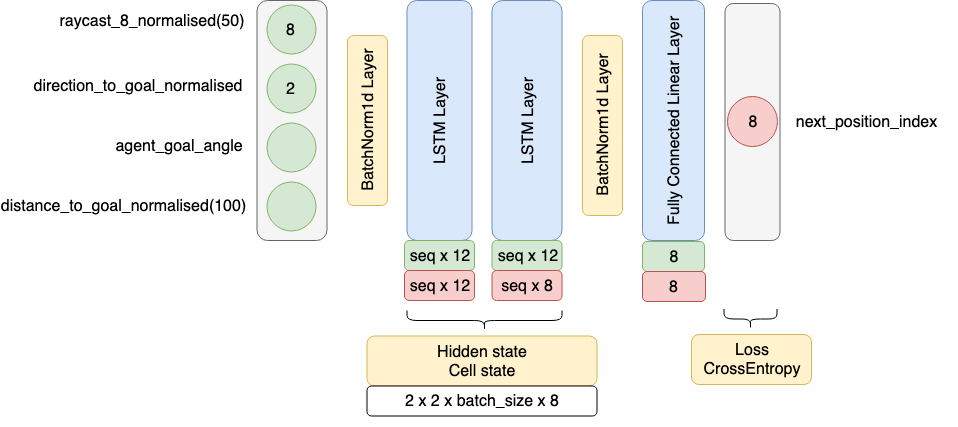
\includegraphics[scale=0.45]{images/lstm_kernel.png}
    \caption{LSTM architecture overview}
    \label{fig:lstm_kernel}
\end{figure}

\textbf{LSTM Layer.} This is the core layer of the network. The layer accepts packed/unpacked sequence data as input, but packed data yields a range of advantages including a training performance boost and input masking which reduces the probability of a preferential action (the exact details are provided in Appendix \ref{sec: app_methods}). We are using two layers as we have to learn non-linear data.

\textbf{Linear Layer.} This is a standard layer from a neural network which contains $n$ weights and one bias. The layer is added to the end of the network to convert the output of the LSTM to an action.

The algorithm itself is trivial as we only need to extract the mentioned features from the map by using the \textbf{MapProcessing} utility class, feed one tensor at a time and execute the given action. The algorithm takes two additional inputs: $model\_name$ and $max\_it$ (with default value $\infty$). The $model\_name$ specifies which model has to be loaded (because the model save name is based on the training set name, we can choose which model we want to use based on the dataset on which it was trained). The $max\_it$ argument states the maximum number of iterations after which the algorithm exits, even if it has not found a path. Before running the main loop, the model has to initialise the hidden and cell state with a 0 tensor of shape $2 \times 2 \times 1 \times 8$ ($batch\_size$ is 1). Sometimes the network will start to oscillate between two points if it cannot find a path (even if one exists). In order to avoid running the algorithm forever, we have implemented a fail-safe mechanism. If a location is visited more than 5 times the algorithm is considered stuck, and it aborts the execution (See Algorithm \ref{alg: lstm}).

%\newpage

\begin{algorithm}[h!]
\caption{Online LSTM Planner}
\label{alg: lstm}
\begin{algorithmic}[1]
\Procedure{Online-LSTM-Planner}{$M\colon(A, Os, G)$, $model\_name$, $max\_it=\infty$}
    \State $model \gets $ load model with save name $model\_name$
    \State Initialise $model$ hidden and cell state with a 0 tensor of shape $2 \times 2 \times 1 \times 8$
    \State $history\_frequency \gets \{\colon\}$
    \State
    \For {$i$ in [0, $max\_it$)}
        \If {G was reached}
            \State \Return
        \EndIf
        %\State
        \State $features \gets$ extract feature tensor from $M$ by using \textbf{MapProcessing} utility class
        \State $next\_action \gets$ $model.forward($features$)$
        %\State
        \If {$next\_action$ is valid}
            \State Move agent $A$ according to $next\_action$
        \EndIf
        \State
        \State $history\_frequency[A] \gets$ 1 (if no value) or $history\_frequency[A] + 1$
        %\State
        \If {history\_frequency[A] > 5}
            \State \Return
        \EndIf
    \EndFor
\EndProcedure
\end{algorithmic}
\end{algorithm}

\subsection{Complexity Analysis}

\begin{Theo}{2-dimensional Complexity}{1_2d_complex}
Worst case time complexity (2D environments; See \Cref{Th:1_1_2d_complex_general} for proof):

\begin{align*}
    \mathcal{O}(OnlineLSTM) = \mathcal{O}(xo + \min(max\_it, d))
\end{align*}

Worst case space complexity (2D environments; See \Cref{Th:1_2_2d_complex_general} for proof):

\begin{align*}
    \mathcal{O}(OnlineLSTM) = \mathcal{O}(1)
\end{align*}

where $xo$ is the inflation pre-process from \textbf{DenseMap} (this is also present in A* when it is run on a \textbf{DenseMap}), $x$ is the inflation rate, $o$ is the average obstacle size and $d$ is the solution depth. 

%where $xo$ is the inflation pre-process from \textbf{DenseMap} (this is also present in A* when it is run on a \textbf{DenseMap}), $x$ is the inflation rate and $o$ is the average obstacle size and $d$ is the solution depth. 
\end{Theo}

% mention special case

\begin{Theo}{D-dimensional Complexity}{1_dd_complex}
Higher dimensional worst case time complexity:

\begin{align*}
    \mathcal{O}(OnlineLSTM) = \mathcal{O}(xo + \min(max\_it, d)\,3^D)
\end{align*}

Higher dimensional worst case space complexity:

\begin{align*}
    \mathcal{O}(OnlineLSTM) = \mathcal{O}(3^D)
\end{align*}

where $xo$ is the inflation pre-process from \textbf{DenseMap} (this is also present in A* when it is run on a \textbf{DenseMap}), $x$ is the inflation rate, $o$ is the average obstacle size, $d$ is the solution depth and $D$ is the dimension size. 

\begin{Proof}{}{test}
In higher dimensions, raycasting is increased to the number of edges in the dimension. Thus, in a 3D world we need 26 raycasts instead of 8. $\mathcal{O}(raycast\_8\_normalised(50))$ becomes $\mathcal{O}(raycast(D, 50)) = \mathcal{O}(3^D \times 50) = \mathcal{O}(3^D)$. Thus, the worst case time complexity becomes $\mathcal{O}(OnlineLSTM) = \mathcal{O}(xo + \min(max\_it, d)\,3^D)$ and the worst case space complexity becomes $\mathcal{O}(OnlineLSTM) = \mathcal{O}(3^D)$.
\end{Proof}

\end{Theo}

\begin{Theo}{General 2-dimensional Worst Case Time Complexity}{1_1_2d_complex_general}
The general worst case time complexity (2D environments) is:

\begin{align*}
    \mathcal{O}(OnlineLSTM) = \mathcal{O}(xo + \min(max\_it, d)\,(\mathcal{O}(collision\_detection) + \\ \mathcal{O}(movement\_action) + \\ \mathcal{O}(feature\_extraction) + \\ \mathcal{O}(network\_pass)))
\end{align*}

where $xo$ is the inflation pre-process from \textbf{DenseMap} (this is also present in A* when it is run on a \textbf{DenseMap}), $x$ is the inflation rate, $o$ is the average obstacle size and $d$ is the solution depth. 

\begin{Proof}{}{test}
$\mathcal{O}(collision\_detection)$ is $\mathcal{O}(1)$ as we are using the \textbf{DenseMap} component. 

$\mathcal{O}(movement\_action)$ (moving the agent to an adjacent location) is $\mathcal{O}(1)$.

\begin{align*}
    \mathcal{O}(feature\_extraction) = \mathcal{O}(\mathcal{O}(raycast\_8\_normalised(50)) + \\ \mathcal{O}(direction\_to\_goal\_normalised) + \\ \mathcal{O}(agent\_goal\_angle) + \\ \mathcal{O}(distance\_to\_goal\_normalised(100)))
\end{align*}

$\mathcal{O}(raycast\_8\_normalised(50))$ is $\mathcal{O}(8 \times 50) = \mathcal{O}(1)$ (one raycast is $\mathcal{O}(n)$, in our case $n=50$ and we compute 8 raycasts; it should be noted that this operation is a bit more expensive in practice, but it is bounded).

\begin{align*}
    \mathcal{O}(direction\_to\_goal\_normalised) &= \mathcal{O}(agent\_goal\_angle) \\ &= \mathcal{O}(distance\_to\_goal\_normalised(100)) \\ &= \mathcal{O}(1)
\end{align*}

Therefore, $\mathcal{O}(feature\_extraction)$ is $\mathcal{O}(1)$.

\begin{align*}
    \mathcal{O}(network\_pass) = \mathcal{O}(\mathcal{O}(packing) + \mathcal{O}(unpacking) + \\ 2\mathcal{O}(batch\_norm) + 2\mathcal{O}(lstm) + \mathcal{O}(linear))
\end{align*}

$\mathcal{O}(packing) + \mathcal{O}(unpacking)$ is $\mathcal{O}(n\log n)$ (in our case $n=1$ so complexity is $\mathcal{O}(1)$).
\\

$\mathcal{O}(batch\_norm)$ is $\mathcal{O}(n)$ where $n$ is the size of the 1D tensor (in our case $n = 12$ and $8$; $\mathcal{O}(12) = \mathcal{O}(8) = \mathcal{O}(1)$, so batch normalisation pass is $\mathcal{O}(1)$). 
\\

$\mathcal{O}(linear)$ is $\mathcal{O}(batch\_size \times input\_size \times output\_size)$ (matrix multiplication) (in our case, $batch\_size = 1$, $input\_size = 8$ and $output\_size = 8$, so $\mathcal{O}(linear) = \mathcal{O}(8 \times 8) = \mathcal{O}(1)$). $\mathcal{O}(lstm)$ is $\mathcal{O}(sequence\_size \times \mathcal{O}(linear))$, but in our case $sequence\_size = 1$ and therefore $\mathcal{O}(lstm) = \mathcal{O}(1)$. 
\\

Lastly, $\mathcal{O}(network\_pass) = \mathcal{O}(1)$ (it should be noted that even if time complexity is $\mathcal{O}(1)$, this operation takes a bit of time, but it is bounded). 
\end{Proof}

\end{Theo}

\begin{Theo}{General 2-dimensional Worst Case Space Complexity}{1_2_2d_complex_general}
The general worst case space complexity (2D environments) is:

\begin{align*}
    \mathcal{O}(OnlineLSTM) = \mathcal{O}(\mathcal{O}(model\_size) + \mathcal{O}(map\_features) + \mathcal{O}(network\_pass) + \\ \mathcal{O}(hidden\_cell\_state))
\end{align*}

\begin{Proof}{}{test}
$\mathcal{O}(model\_size)$ is the loaded model architecture size which can be treated as $\mathcal{O}(1)$.
\\

$\mathcal{O}(map\_features)$ is $\mathcal{O}(12) = \mathcal{O}(1)$ (we extract 12 features: 8 raycast\_8\_normalised(50), 2 direction\_to\_goal\_normalised, 1 agent\_goal\_angle, 1 distance\_to\_goal\_normalised(100)). 
\\

$\mathcal{O}(network\_pass)$ is the maximum size of the transformed input which is $\mathcal{O}(12) = \mathcal{O}(1)$. 
\\

$\mathcal{O}(hidden\_cell\_state)$ is $\mathcal{O}(2 \times lstm\_layers \times batch\_size \times lstm\_output\_size)$ (in our case, $\mathcal{O}(hidden\_cell\_state)$ = $\mathcal{O}(2 \times 2 \times 1 \times 8) = \mathcal{O}(1)$). 
\end{Proof}

\end{Theo}

\subsection{General Discussion}

This solution does not usually find the optimal path, but it is relatively close to the performance of A*. When running the algorithm in simple environments (maps that contain several simple obstacles that resemble primitives (circles, squares) with/without clear sections (areas where the path is not obstructed by any obstacle)) the optimal performance is equal (most of the time) or insignificantly smaller than A*.

A major advantage over A* is that this method uses significantly less memory as no exploration is done ($\mathcal{O}(OnlineLSTM) = \mathcal{O}(1)$ < $\mathcal{O}(A*) =  \mathcal{O}(\hat{b}^d)$) (See Figure \ref{fig: lstm path success}). When the map size is small ($64 \times 64$) the algorithm is usually slower than A*, due to the feature extraction and network pass, but when the map size gets bigger ($600 \times 600$ after empirical run, but could be smaller), as it usually is the case in the real world, the algorithm is faster than A* (and will be for larger maps as well). This is intuitively and theoretical correct as we can notice that if we inspect the complexities of both algorithms: $\mathcal{O}(Online LSTM) = \mathcal{O}(xo + \min(max\_it, d)) < \mathcal{O}(A*) = \mathcal{O}(xo + \hat{b}^d)$. The exponential time and space complexity increase in higher dimensions is reduced as well (time: $\mathcal{O}(Online LSTM) = \mathcal{O}(xo + \min(max\_it, d)\,3^D) < \mathcal{O}(A*) = \mathcal{O}(xo + (3^D)^d)$, space: $\mathcal{O}(OnlineLSTM) = \mathcal{O}(3^D)$ < $\mathcal{O}(A*) = \mathcal{O}((3^D)^d)$). It should be noted that A* still reduces the time and space complexity even in higher dimensions ($\mathcal{O}(\hat{b}^d) < \mathcal{O}((3^D)^d$), but it highly depends on the heuristic choice. Lastly, the algorithm is online (supports external updates to the internal state), meaning that it supports dynamic and partial knowledge environments, unlike A*.

By following the paper implementation, we have inherited some issues. The major drawback is that the algorithm is quite greedy (due to the nature of the A* heuristic) and it does not know how to go around big obstacles and long corridors. Therefore, when the environment contains complex obstacles, the algorithm might not find a path to the goal (See Figure \ref{fig: lstm path fail}). Moreover, it is quite hard to infer the obstacle shape from the model input and adding more hard-coded features to describe the shape of the obstacle (e.g. the length of the obstacle boundary, the bounding box size of the obstacle and so on) is not feasible and increases the computational cost.

\pagebreak

% Original size was 0.4

\begin{figure}[h!]
  %\centering
  \centerfloat
  \begin{subfigure}[b]{0.33\linewidth}
    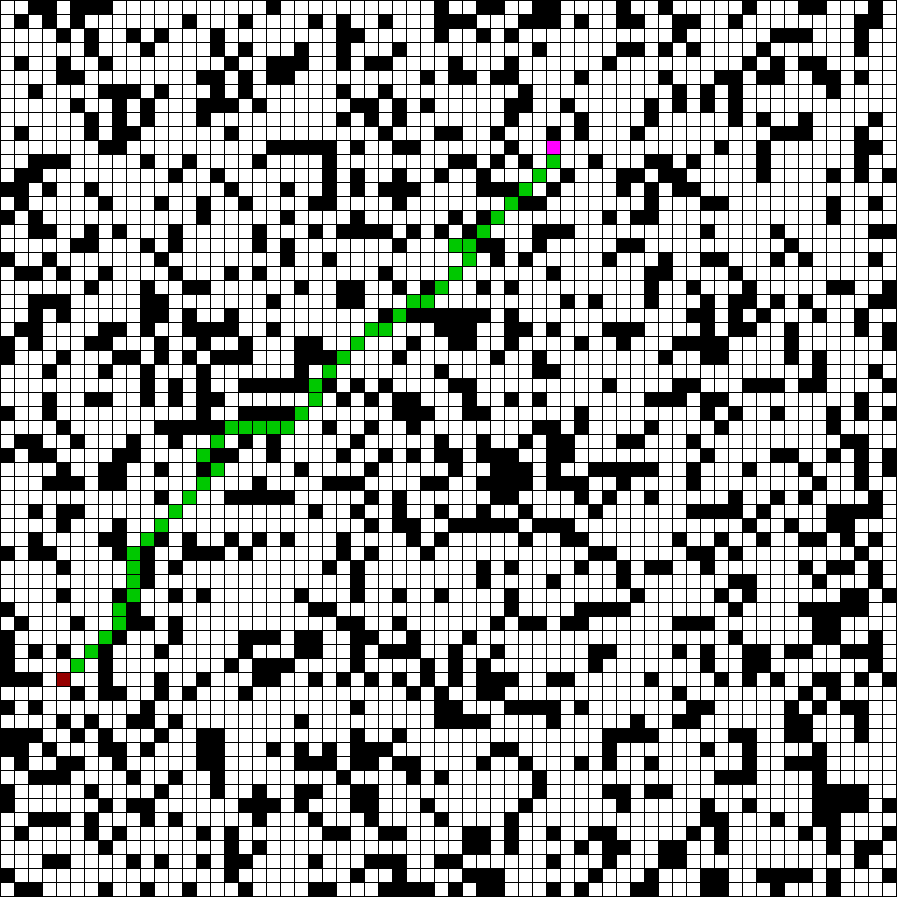
\includegraphics[width=\linewidth]{images/lstm_1_all.png}
     \caption{Goal found}
  \end{subfigure}
  \hfill
  \begin{subfigure}[b]{0.33\linewidth}
    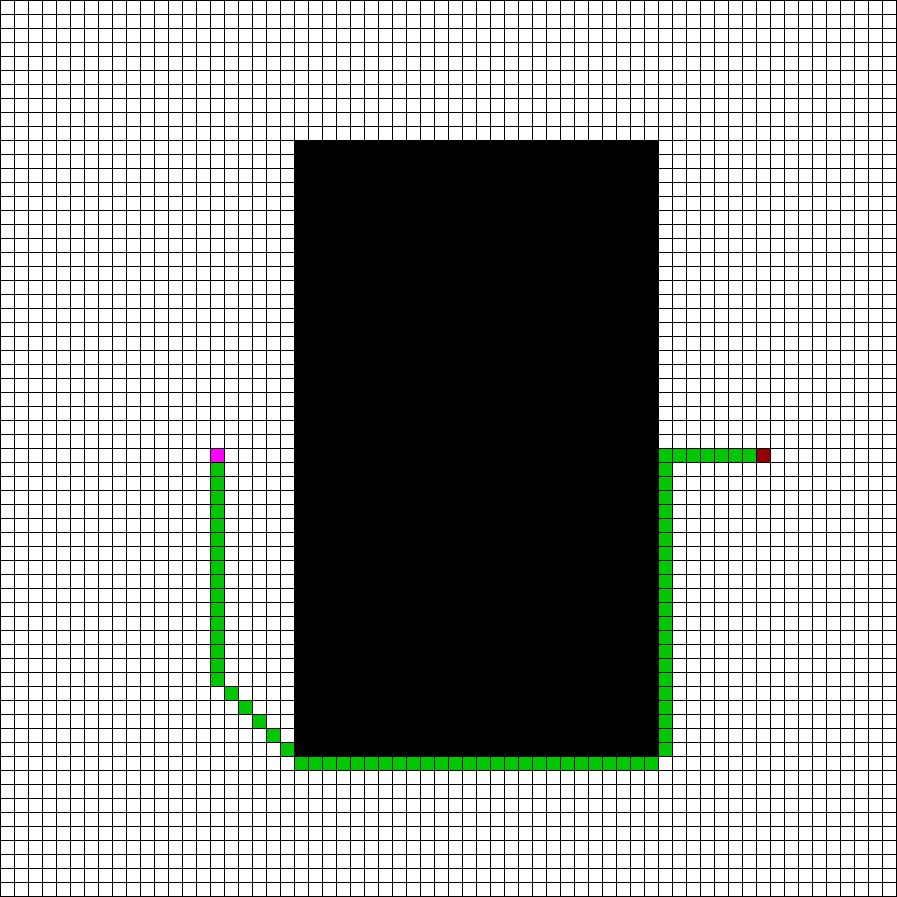
\includegraphics[width=\linewidth]{images/lstm_2_all.png}
     \caption{Goal found}
  \end{subfigure}
  \hfill
  \begin{subfigure}[b]{0.33\linewidth}
    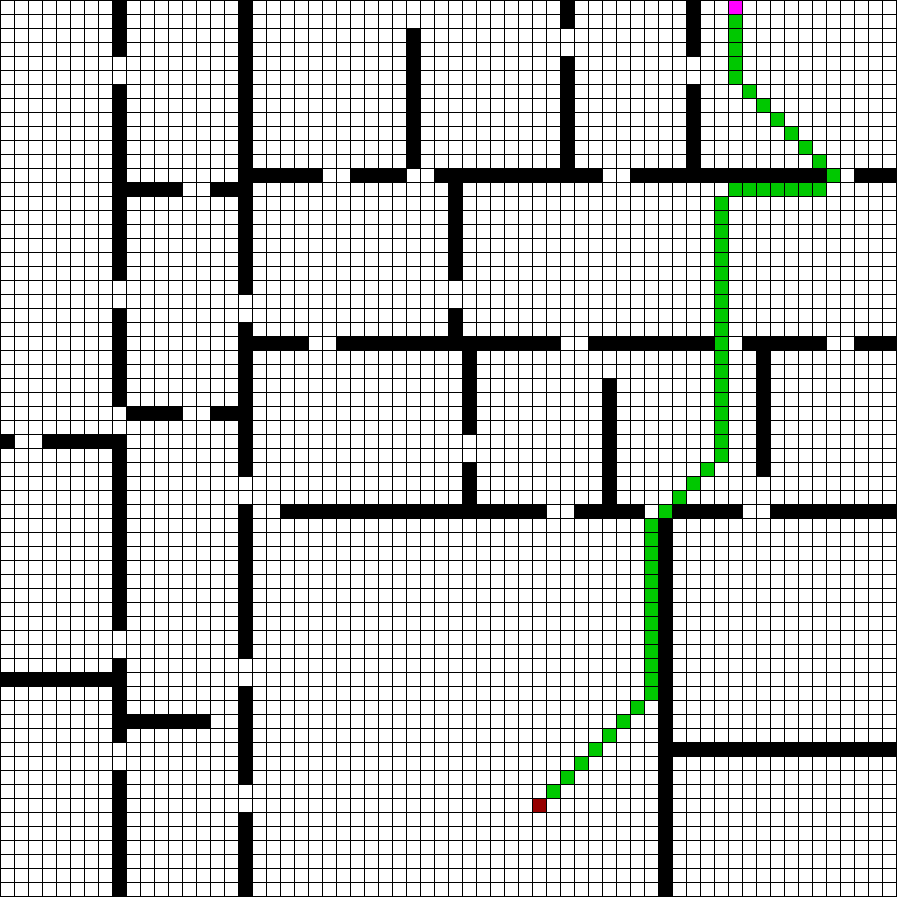
\includegraphics[width=\linewidth]{images/lstm_3_all.png}
     \caption{Goal found}
  \end{subfigure}
  \caption{Successful Online LSTM Planner trained on all 30000 generated maps paths}
  \label{fig: lstm path success}
\end{figure}

\begin{figure}[h!]
  \centerfloat
  \begin{subfigure}[b]{0.33\linewidth}
    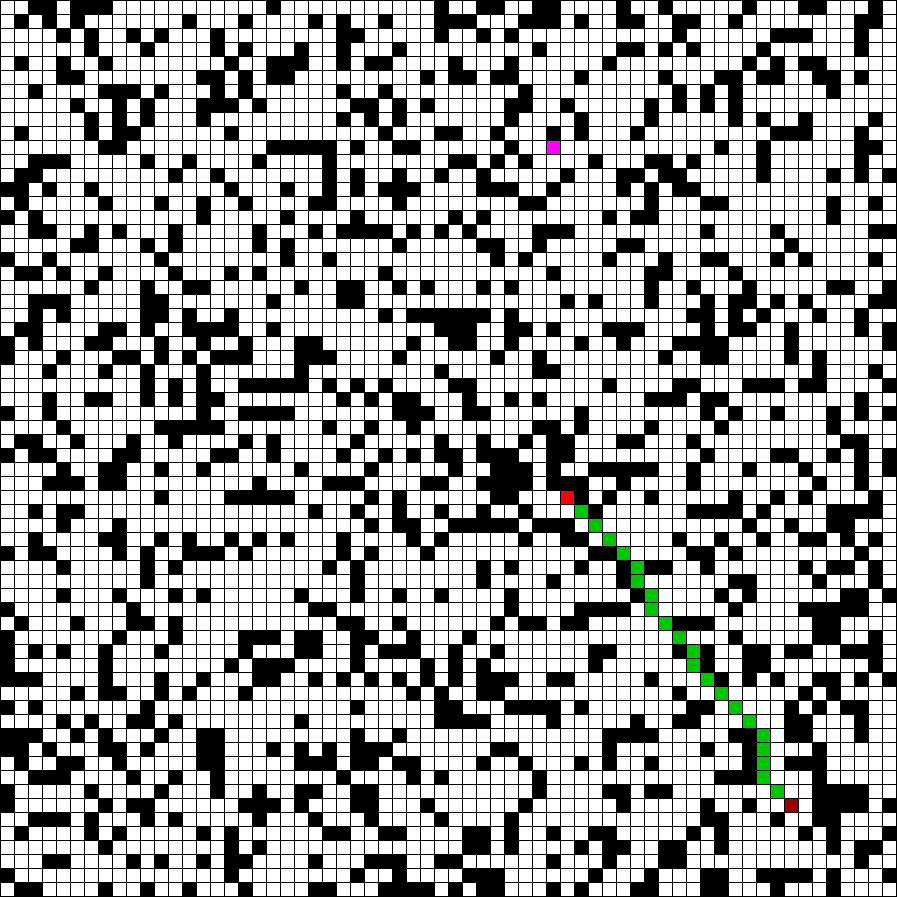
\includegraphics[width=\linewidth]{images/lstm_1_all_fail.png}
     \caption{Goal not found \newline}
  \end{subfigure}
  \hfill
  \begin{subfigure}[b]{0.33\linewidth}
    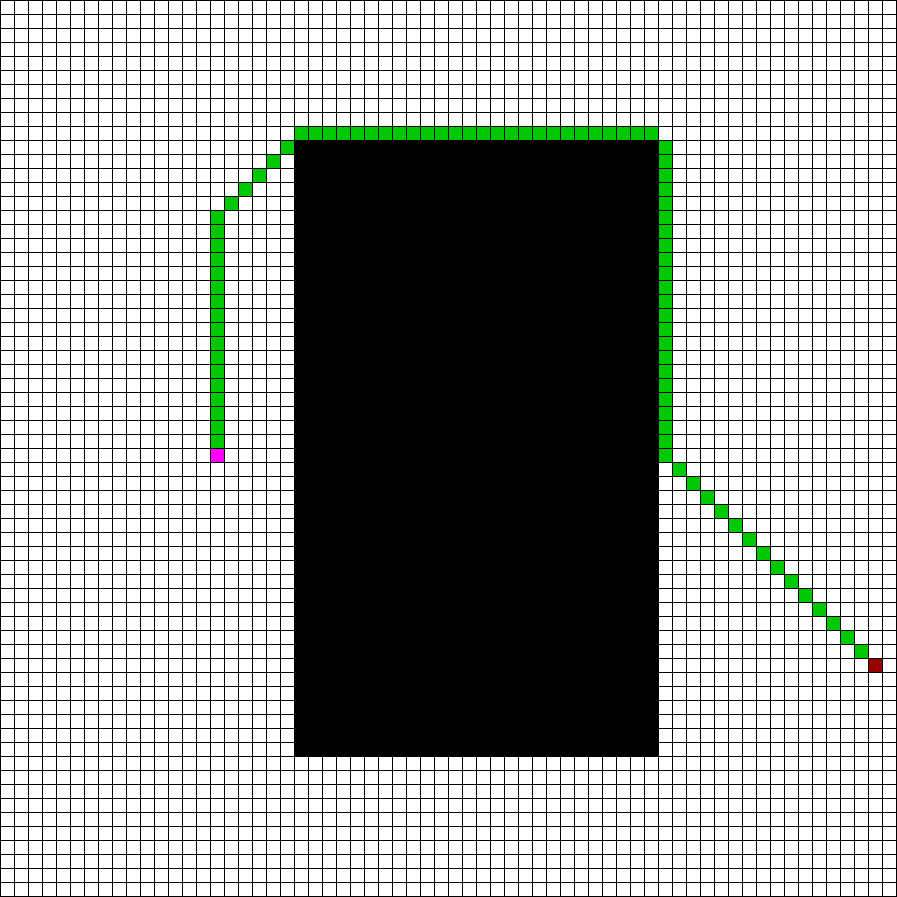
\includegraphics[width=\linewidth]{images/lstm_2_all_fail.png}
     \caption{Path too long \newline}
  \end{subfigure}
  \hfill
  \begin{subfigure}[b]{0.33\linewidth}
    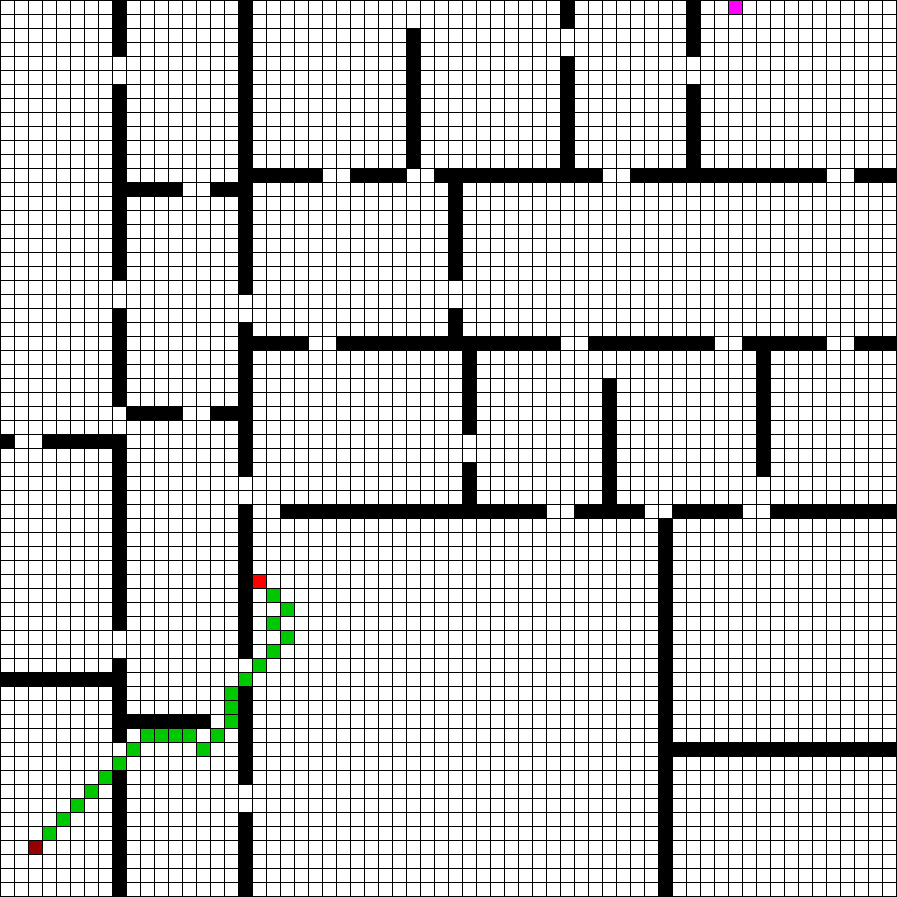
\includegraphics[width=\linewidth]{images/lstm_4_all.png}
     \caption{Goal not found due to long corridors}
  \end{subfigure}
  \caption{Failed Online LSTM Planner 
  trained on all 30000 generated maps paths}
  \label{fig: lstm path fail}
\end{figure}

\pagebreak

\section{CAE Online LSTM Planner}

The Convolutional Auto-encoder (CAE) Online LSTM Planner is a hybrid architecture based on the Online LSTM Planner and \cite{inoue2019robot}. The algorithm attempts to solve the big obstacle navigation issue mentioned in the previous section by supplying extra features that describe the environment to the model (the global image snapshot). This is done by using a Convolutional Auto-encoder (CAE) to encode the global map features and feed the encoder output to the LSTM model (See Figure \ref{fig:caelstm_full}).

\begin{figure}[h!]
    \centering
    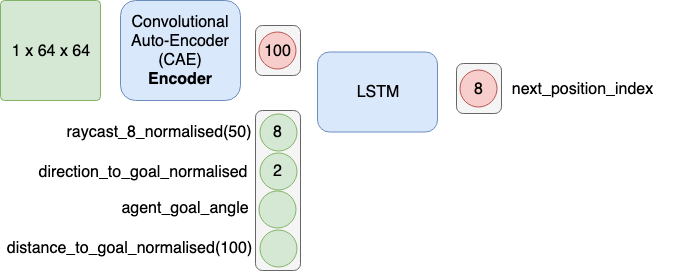
\includegraphics[scale=0.5]{images/caelstm_full.png}
    \caption{CAE and LSTM network architecture overviews}
    \label{fig:caelstm_full}
\end{figure}

\subsection{CAE Architecture}

In order to avoid obstacle hard-coded features, we can make use of a CAE \cite{holden2015learning, ml} or Principal Component Analysis (PCA) \cite{jolliffe2011principal, wold1987principal} model to extract the most representative features from the global map. Thus, we save computational performance and we do not need to manually examine each obstacle. The CAE was chosen over PCA as the training pipeline had to be slightly modified to feed the batched input to the PCA by following a similar approach to the \textbf{IncrementalPCA} model from \textit{sklearn}. Moreover, if batches were removed, we would have probably run out of memory as the training set is quite large (500 MB for 10000 $64\times64$ uniform random fill maps). Lastly, \cite{inoue2019robot} has achieved great success rate results by using a CAE.

We have chosen a Convolutional Auto-encoder (AE) instead of a normal Linear AE because we would like to learn reproducible patterns from the input image. By creating convolution layers we learn different sets of localised patterns in the image \cite{holden2015learning, ml}.

The CAE is trained on the map training datasets, but it can also be trained on different standard datasets such as MNIST \cite{mnist} (implemented), CIFAR-10 \cite{cifar_10} (can be extended). The CAE includes a specialised results display procedure. Depending on the training dataset, it displays two plots with row size equal to the number of different classes of maps and each row contains three images: the original image, the reconstructed version and the latent space viewed as a 2D grey scale image (the latent space is reshaped). The reason why we display two plots is that we would like to inspect how the latent space varies on maps that are within the same class. It also applies the same procedure if the MNIST dataset is used instead, but it only displays one plot with the first three samples. Furthermore, we plot the feature maps (each convolution output) for the three types of maps.

%\todo{Latent space vriation??}
% The performance of the CAE is assessed by comparing the input and output images and computing the loss between them (L1 loss was used to compare the two images)

The CAE model architecture contains two sections: the Encoder and the Decoder (See Figure \ref{fig:caelstm_all_sections}). The CAE uses the L1 loss function:

$$L(\boldsymbol{x}, \boldsymbol{y}) = \norm{\boldsymbol{x} - \boldsymbol{y}}_{1}\textrm{, where \boldsymbol{x} is the prediction and \boldsymbol{y} is the target}$$

The scope of the CAE is to compress the given image into a small sized vector (the latent space) which contains the most significant features of the image and then reconstruct it back. We pre-process the data by normalising the image with mean 0.5 and standard deviation 0.5. Thus, the input is in the range [-1, 1]. We provide a flag that enables or disables skip connections between a convolution and the mirror de-convolution. By using skip-connection, we make use of the data that was lost during compression to reconstruct the image and thus, the performance improves (the Encoder learns more information as well).

\begin{figure}[h!]
    \centerfloat
    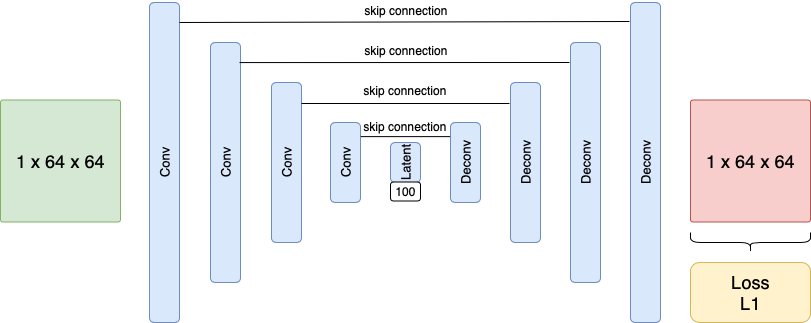
\includegraphics[scale=0.5]{images/caelstm_all_sections.png}
    \caption{CAE model architecture overview}
    \label{fig:caelstm_all_sections}
\end{figure}

The CAE Encoder contains four convolutional layers and one linear layer as seen in Figure \ref{fig:caelstm_section_cae_kernel_encoder}. Each convolution layer is composed of multiple layers placed in this following order: convolutional layer, batch normalisation layer, max pool and leaky ReLU as the activation function. The final layer of the encoder is a linear layer with another batch normalisation layer. 

\begin{figure}[h!]
    \centerfloat
    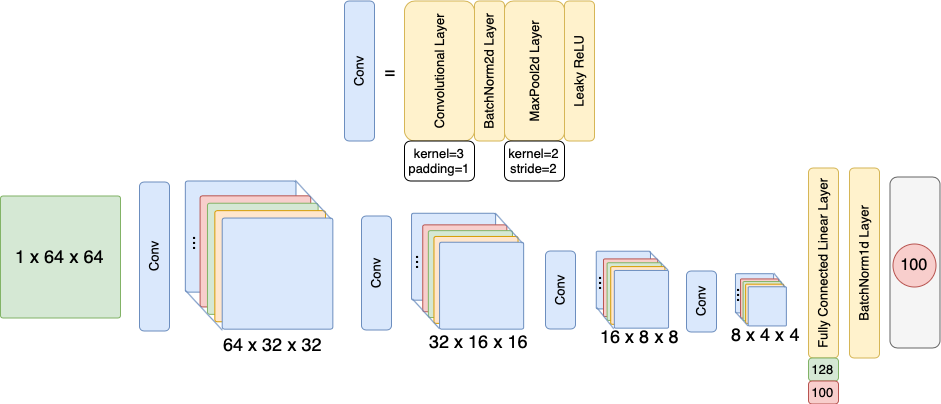
\includegraphics[scale=0.45]{images/caelstm_section_cae_kernel_encoder.png}
    \caption{CAE Encoder architecture}
    \label{fig:caelstm_section_cae_kernel_encoder}
\end{figure}

\textbf{Convolutional Layer.} The convolutional layer uses a kernel window with learnable weights and bias, which is applied to the input image to extract the localised features. In our model, the kernel window has $(c)\times(i)\times3\times3$ dimension where $c$ is the number of output channels, and $i$ is the number of input channels (the window is applied to all input channels). The padding parameter defines how much the image is padded with 0s (in our case, we have 1 padding for all convolutions). The stride parameter defines how much the kernel window is shifted along the image (in our case, we use the default value 1). By using a $3\times3$ kernel and 1 padding, we preserve the image dimensions and change the number of channels.

\textbf{Batch Normalisation Layer.} We use batch normalisation layers for the same reason described in the the Online LSTM Planner.

\textbf{Max Pool.} The max pool layer has the same arguments as the convolutional layer (kernel, padding, stride), but the kernel has no learnable parameters. By using a max pool layer with kernel size 2, padding 0 and stride 2, we reduce the image dimension by half. Max pooling is applied to all channels and thus, the number of output channels is identical to the number of input channels.

\textbf{Leaky ReLU.} The activation function breaks the linearities between two layers. Thus, the layers cannot be collapsed into a single layer. The Leaky ReLU function ($f(x) = \begin{cases} a \cdot x, x < 0 \\ x,\,\,\,\,\,\,\,\, x \geq 0 \end{cases}$) is a modified version of the ReLU function which allows clamped negative values. The variable that defines the clamping ($a$) is a learnable parameter, and it is updated during back-propagation. After running a series of empirical evaluations on the training routine, we have decided to use Leaky ReLU (instead of ReLU) as the extra learnable parameter has improved the overall performance of the network.

\textbf{Linear Layer.} We include a linear layer at the end to convert the final image (by reshaping it along with all channels) into the latent vector.

The CAE Decoder contains one linear layer and four de-convolutional layers as seen in Figure \ref{fig:caelstm_section_cae_kernel_decoder}.  Each de-convolutional layer is composed of multiple layers placed in the following order: de-convolutional layer, batch normalisation layer (used for the same reason as described above) and ReLU activation function. The last de-convolutional layer has Tanh activation function as the input is normalised in the range [-1, 1] and the output of Tanh matches it.

\begin{figure}[h!]
    \centerfloat
    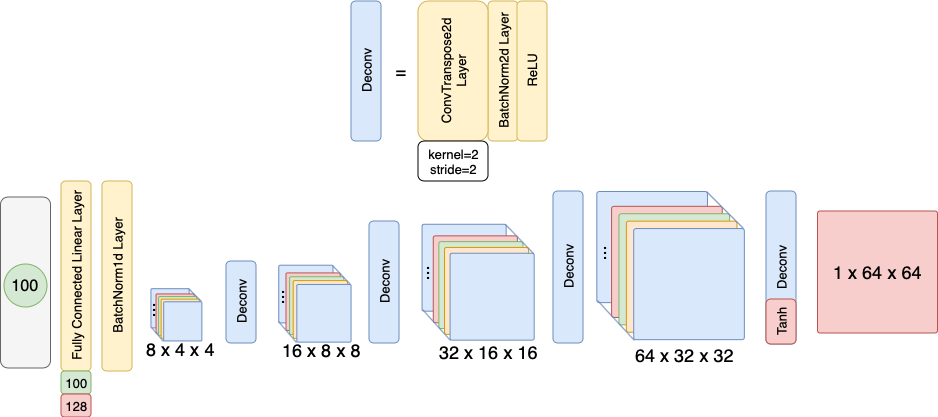
\includegraphics[scale=0.45]{images/caelstm_section_cae_kernel_decoder.png}
    \caption{CAE Decoder architecture}
    \label{fig:caelstm_section_cae_kernel_decoder}
\end{figure}

\textbf{Linear Layer.} The initial linear layer converts the latent space back to the compressed image.

\textbf{De-convolutional Layer.} De-convolution is achieved by using the \textbf{ConvTranspose2d} module (kernel size 2, stride 2, padding 0) from \textit{pytorch}. It represents the inverse operation of a convolution and, in our case, it acts as a layer that contains a convolutional layer with max pool that increases the image size by half (instead of reducing it).

\textbf{ReLU.} Again, after running empirical evaluations, we have noticed that ReLU achieves better performance. Moreover, by not allowing negative values, we force the encoder to learn and the network will not reconstruct the image only from the decoder (by having a 0 latent space).

\pagebreak

\subsection{LSTM Architecture}

The LSTM network is identical to the LSTM architecture of the Online LSTM Planner and uses the same loss function (cross entropy loss). The only difference is that we feed the CAE Encoder output along with all inputs of the LSTM network (See Figure \ref{fig:caelstm_section_lstm_kernel}). We define a different model because we have to pre-process the input and join sequence data with single global images. Global images are replicated $n_i$ times where $n_i$ is the sequence length of sample $i$. Afterwards, the images are sorted according to the permutation that was used to sort the sequence input and joined together into a single tensor feature (per sample, per sequence).

\begin{figure}[h!]
    \centerfloat
    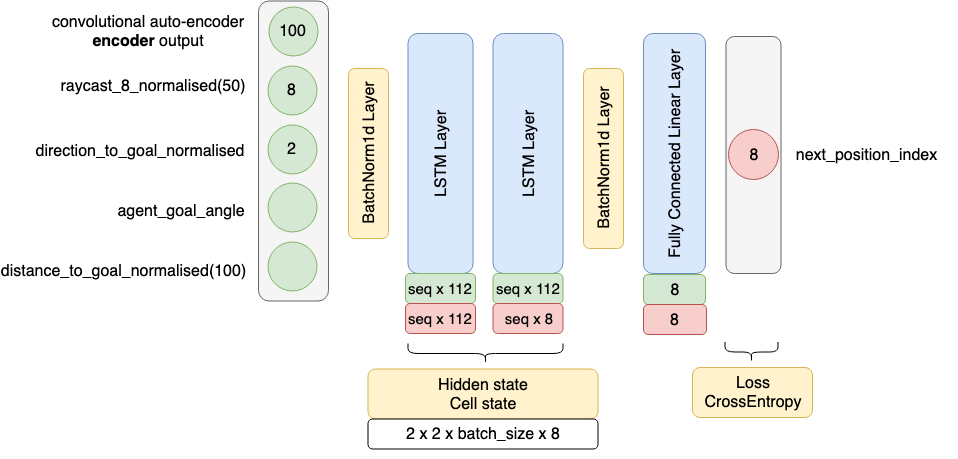
\includegraphics[scale=0.45]{images/caelstm_section_lstm_kernel.png}
    \caption{LSTM network architecture overview}
    \label{fig:caelstm_section_lstm_kernel}
\end{figure}

The algorithm itself is identical to the Online LSTM Planner (See Algorithm \ref{alg: lstm}), but we load the LSTM model associated with this planner instead. When we load the LSTM model, we cache the \textbf{encoded} global map snapshot scaled to $64\times64$ size (regardless if it is smaller or bigger). At each LSTM network pass, we concatenate the cached encoded map to the extracted features. It should be noted that the algorithm is theoretically online as it uses the same model as the Online LSTM Planner. However, because we cache the map in the beginning to increase the time performance, the algorithm might have inferior execution results when we discover more areas within the map. A simple solution to maintain the same performance as the Online LSTM Planner would be to take global map snapshots at each time step instead of caching the first result, while trading time efficiency. Nonetheless, we have made this choice due to the design of the final proposed solution, Global Way-point LSTM Planner.

%As a possible memory optimisation we can only take the localised 64x64 map when the map size is bigger than 64x64 (this is valid as the network was trained on normalised inputs; we learn the data distribution, not the actual data itself), but this operation cannot be cached and has to be executed at each feature extraction step.

\newpage

\subsection{Complexity Analysis}

\begin{Theo}{2-dimensional Complexity}{2_2d_complex}
Worst case time complexity (2D environments; See \Cref{Th:2_1_2d_complex_general} for proof):
\begin{align*}
    \mathcal{O}(CAEOnlineLSTM) = \mathcal{O}(xo + nm \log nm + \min(max\_it, d))
\end{align*}

Worst case space complexity (2D environments; See \Cref{Th:2_2_2d_complex_general} for proof):
\begin{align*}
    \mathcal{O}(CAEOnlineLSTM) = \mathcal{O}(1)
\end{align*}

where $xo$ is the inflation pre-process from \textbf{DenseMap} (this is also present in A* when it is run on a \textbf{DenseMap}), $x$ is the inflation rate, $o$ is the average obstacle size, $d$ is the solution depth and $n$, $m$ are the global image snapshot dimensions.

\end{Theo}

\begin{Theo}{D-dimensional Complexity}{1_dd_complex}
Higher dimensional worst case time complexity:

\begin{align*}
    \mathcal{O}(CAEOnlineLSTM) = \mathcal{O}(xo + n^D \log n^D + 64^D \log 64^D + \min(max\_it, d)\,3^D)
\end{align*}

Higher dimensional worst case space complexity:

\begin{align*}
    \mathcal{O}(CAEOnlineLSTM) = \mathcal{O}(64^D)
\end{align*}

where $xo$ is the inflation pre-process from \textbf{DenseMap} (this is also present in A* when it is run on a \textbf{DenseMap}), $x$ is the inflation rate, $o$ is the average obstacle size, $d$ is the solution depth, $D$ is the dimension size and $n^D$ is the global image snapshot dimensions

\begin{Proof}{}{test}
In higher dimensions, the global snapshot is increased to $64^D$, where $D$ is the dimension number and the raycasting increase is inherited from the Online LSTM algorithm. $\mathcal{O}(CAE\_pass)$ becomes $\mathcal{O}(64^D \log 64^D)$ and $\mathcal{O}(scaling)$ becomes $\mathcal{O}(n^D \log n^D)$, where $n$ is the average dimension length of the original map. Therefore, the time complexity becomes $\mathcal{O}(CAEOnlineLSTM) = \mathcal{O}(xo + n^D \log n^D + 64^D \log 64^D + \min(max\_it, d)\,3^D)$ (latent space is still 100) and the space complexity becomes $\mathcal{O}(CAEOnlineLSTM) = \mathcal{O}(64^D)$. Moreover, the architecture has to be changed to support higher dimensions by using higher dimension convolutions or reshaping the input. We can notice that is quickly becomes an infeasible solution. A solution would be to decrease the global image size ($64^D$) to something smaller, but since we are dealing with real robots we can stop at 3D dimensions (which is still feasible with the current architecture and 3D convolutions). Furthermore, we can even keep the global image size to $64\times64$ in higher dimensions (by projecting the environment onto a $64\times64$ plane or using PCA). This procedure incurs a performance loss (due to the loss of data in the projection), but achieves better real world applicability.
\end{Proof}
\end{Theo}

\begin{Theo}{General 2-dimensional Worst Case Time Complexity}{2_1_2d_complex_general}
The general worst case time complexity (2D environments) is:

\begin{align*}
    \mathcal{O}(CAEOnlineLSTM) = \mathcal{O}(xo + \mathcal{O}(pre\_process) + \\ \min(max\_it, d)(\mathcal{O}(collision\_detection) + \mathcal{O}(movement\_action) + \\ \mathcal{O}(feature\_extraction) + \mathcal{O}(lstm\_network\_pass)))
\end{align*}

where $xo$ is the inflation complexity and $d$ is the solution depth.

\begin{Proof}{}{test}
$\mathcal{O}(collision\_detection) = \mathcal{O}(movement\_action) = \mathcal{O}(feature\_extraction) = \mathcal{O}(1)$ as in OnlineLSTM (for $\mathcal{O}(feature\_extraction)$ we extract the same old features and concatenate them with the cahced encoded map). 

\begin{align*}
    \mathcal{O}(pre\_process) &= \mathcal{O}(\mathcal{O}(scaling) + \mathcal{O}(CAE\_pass))\\
    \mathcal{O}(CAE\_pass) &= \mathcal{O}(4\mathcal{O}(convolution) + 4\mathcal{O}(deconvolution) + 2\mathcal{O}(linear))
\end{align*}

Kernel based convolutions are realised by making use of the Fast Fourier Transform (FFT) method which is $\mathcal{O}(n \log n)$. Because we encode a $64\times64$ image (the input is bounded) we can consider this to be $\mathcal{O}(CAE\_pass) = \mathcal{O}(1)$ (in practice, this step is quite expensive, but the input is bounded and it is only run once). We can scale using a kernel window (similar to max pooling), in our case scaling is two dimensional and depends on the image size. Therefore the scaling complexity becomes $\mathcal{O}(scaling) = \mathcal{O}(nm \log nm)$, where $n$ is the width and $m$ is the height of the original map image, so $\mathcal{O}(pre\_process)$ = $\mathcal{O}(nm \log nm)$ (the encoded map is cached; encoding is $\mathcal{O}(1)$).
\\

$\mathcal{O}(lstm\_network\_pass)$ takes a 112 sized input (100 encoded latent space and 12 old features), but it is still $\mathcal{O}(1)$ (in practice this takes longer than the OnlineLSTM network pass, but it is bounded). 

\end{Proof}

\end{Theo}

% For local snapshot solution, no pre-processing is used so $\mathcal{O}(pre\_process) = \mathcal{O}(1)$, but $\mathcal{O}(global\_map) = \mathcal{O}(64\times64) = \mathcal{O}(1)$ (simple local iteration), so $\mathcal{O}(feature\_extraction) = \mathcal{O}(1)$.
% and $\mathcal{O}(CAEOnlineLSTM) = \mathcal{O}(xo) + \mathcal{O}(\min(max\_it, d)$ for the local snapshot solution.

% $\mathcal{O}(pre\_process)$ and $\mathcal{O}(global\_map)$ depend on the type of global map extraction: scaling (memory unoptimised), local snapshot (memory optimised).

\begin{Theo}{General 2-dimensional Worst Case Space Complexity}{2_2_2d_complex_general}
The general worst case space complexity (2D environments) is:
\begin{align*}
    \mathcal{O}(CAEOnlineLSTM) = \mathcal{O}(\mathcal{O}(model\_size) + \mathcal{O}(scaling) + \mathcal{O}(map\_features) + \\ \mathcal{O}(cae\_network\_pass) + \mathcal{O}(lstm\_network\_pass) + \mathcal{O}(hidden\_cell\_state))
\end{align*}

\begin{Proof}{}{test}
$\mathcal{O}(model\_size) = \mathcal{O}(map\_featrues) = \mathcal{O}(lstm\_network\_pass) = \mathcal{O}(hidden\_cell\_state) = \mathcal{O}(1)$ as in OnlineLSTM (for $\mathcal{O}(map\_features)$ we have 112 features which is still $\mathcal{O}(1)$).
\\

$\mathcal{O}(scaling)$ is bounded by the scaled image size which is $64\times64$. Therefore, $\mathcal{O}(scaling) = \mathcal{O}(1)$.
\\

$\mathcal{O}(cae\_network\_pass)$ is bounded by the largest feature map in the network, which is $64\times32\times32$ and therefore $\mathcal{O}(cae\_network\_pass) = \mathcal{O}(1)$. 
\end{Proof}
\end{Theo}

% The space complexity is the same as the Online LSTM algorithm which is $\mathcal{O}(1)$. We have 112 features and the combined CAE and LSTM network transformed features does not exceed 64x32x32 features at one time. This property holds for both the memory optimised and memory unoptimised versions.

\subsection{General Discussion}

The CAE Online LSTM Planner shares the same advantages as the Online LSTM Planner. It is quite hard to argue if the implementation is better than A* in time and space complexity as the dimension increases, but it is better on 2D and 3D worlds. Lastly, it is a theoretically online solution, and therefore, it supports dynamic environments and partial knowledge. As mentioned above, in order to make it practically online, we have to feed a new global map snapshot at each time step. Because the extracted map is bounded, the worst case space complexity remains the same, but the worst case time complexity becomes $\mathcal{O}(CAEOnlineLSTM) = \mathcal{O}(xo + \min(max\_it, d)(nm \log nm))$ as we have to extract the global map snapshot and scale it at each time step.

The performance of the algorithm seems to be worse than the Online LSTM overall (See Figure \ref{fig: cae lstm path success}), but it has a significant advantage. The algorithm is less greedy and attempts to go around obstacles more often, but it usually gets lost in the later stages (after a few iterations) (See Figure \ref{fig: cae lstm vs lstm}). This is quite important for the LSTM Bagging Planner from the next section.

% original size was 45

\begin{figure}[h!]
  \centerfloat
  \begin{subfigure}[b]{0.33\linewidth}
    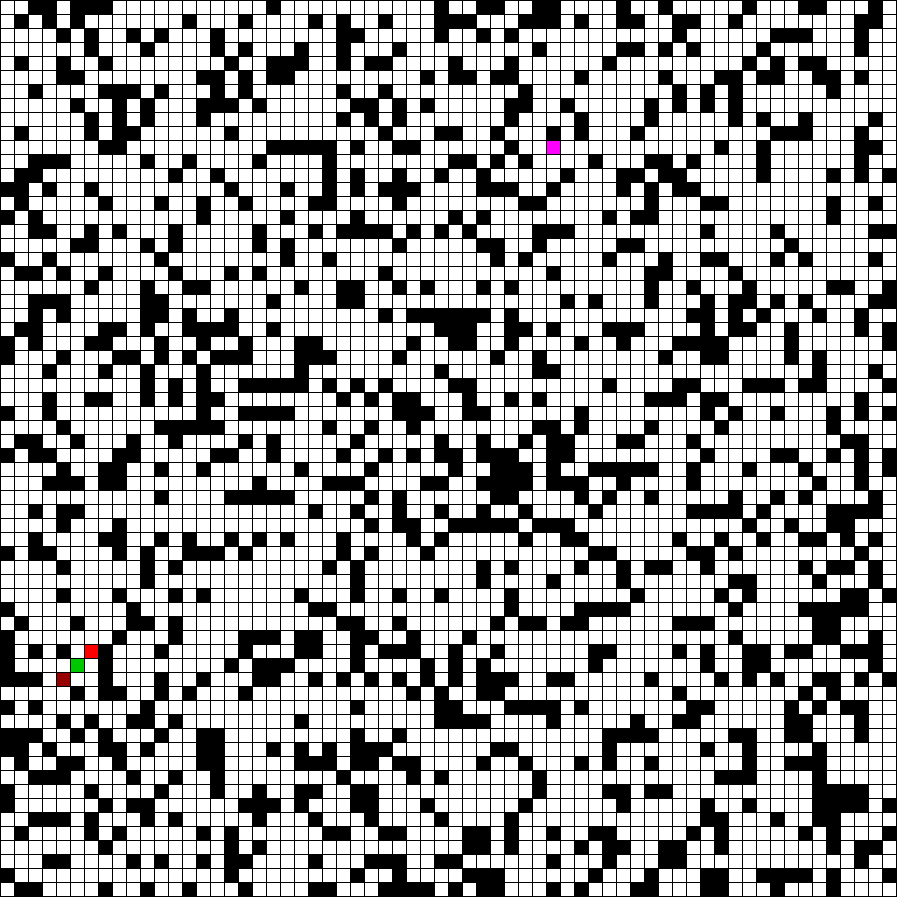
\includegraphics[width=\linewidth]{images/cae_lstm_1_block.png}
     \caption{Goal not found}
  \end{subfigure}
  \hfill
  \begin{subfigure}[b]{0.33\linewidth}
    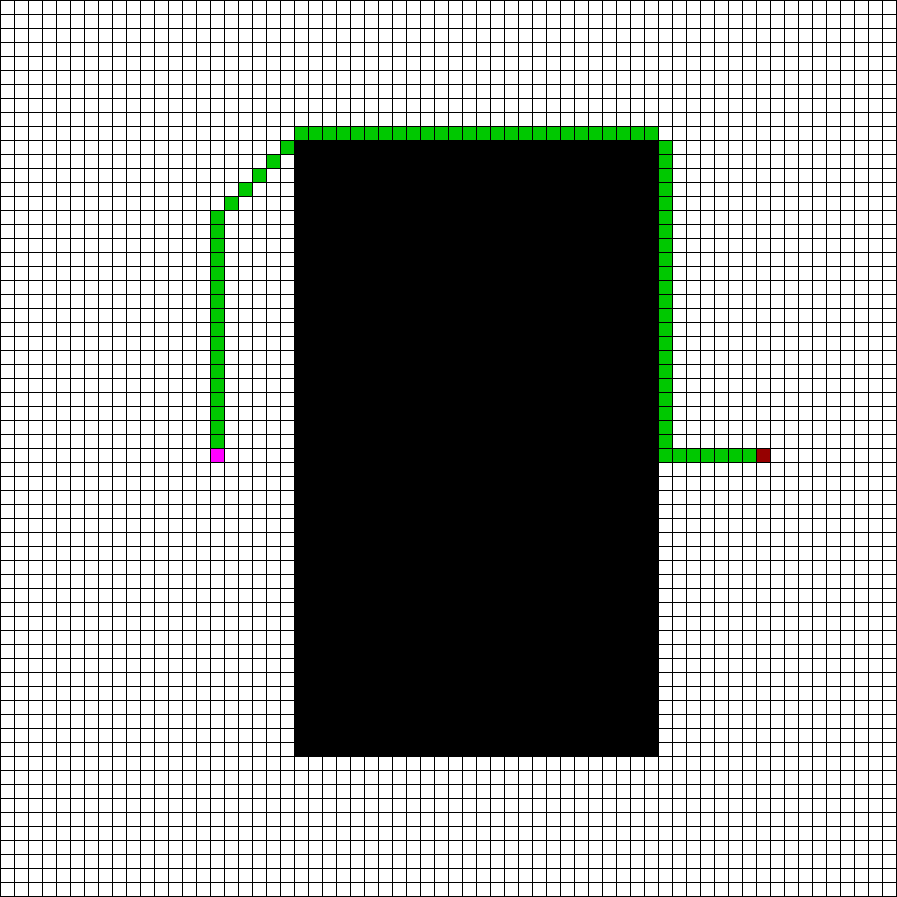
\includegraphics[width=\linewidth]{images/cae_lstm_2_block.png}
     \caption{Goal found}
  \end{subfigure}
  \hfill
  \begin{subfigure}[b]{0.33\linewidth}
    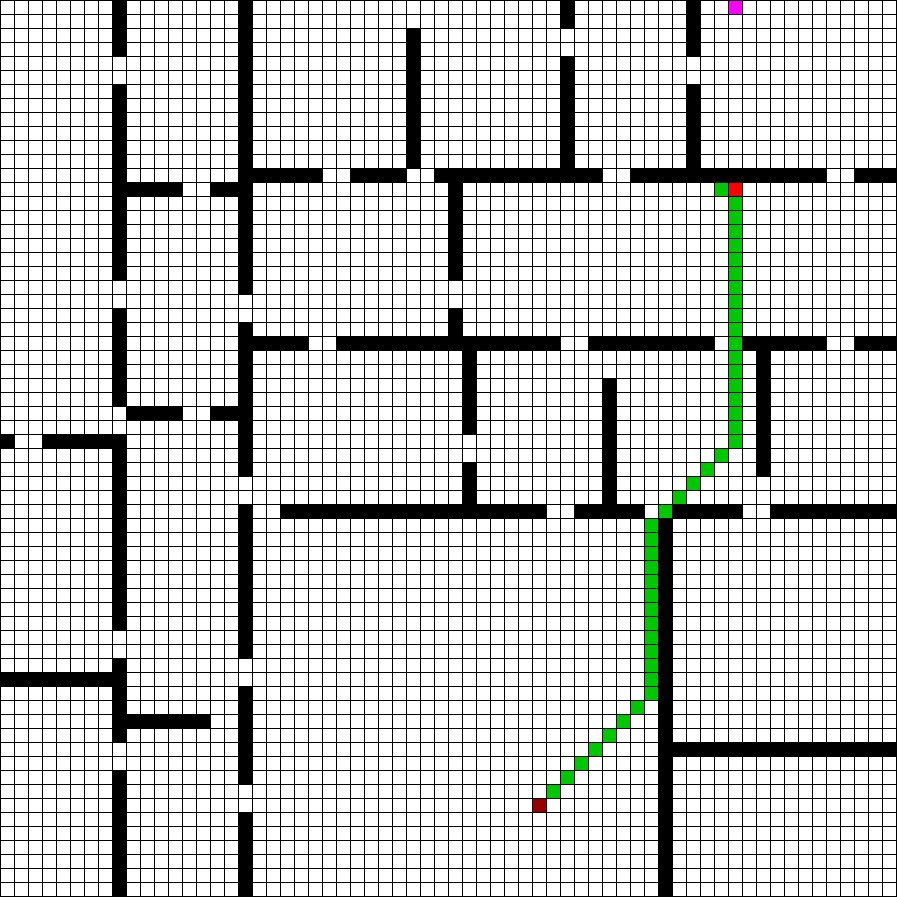
\includegraphics[width=\linewidth]{images/cae_lstm_3_block.png}
     \caption{Goal not found}
  \end{subfigure}
  \caption{CAE Online LSTM Planner trained on 10000 block maps paths. The map agent and goal position are identical to the one from figure \ref{fig: lstm path success}}
  \label{fig: cae lstm path success}
\end{figure}

\begin{figure}[h!]
  \centerfloat
  \begin{subfigure}[b]{0.40\linewidth}
    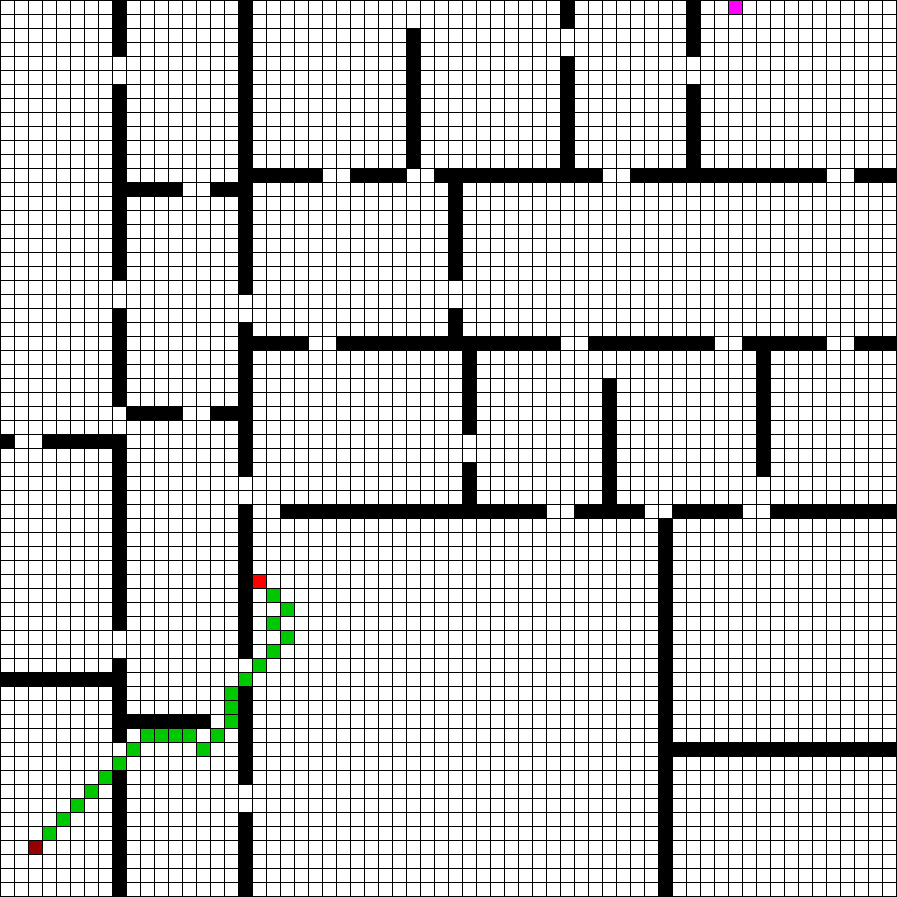
\includegraphics[width=\linewidth]{images/lstm_4_all.png}
     \caption{Online LSTM Planner}
  \end{subfigure}
  \hfill
  \begin{subfigure}[b]{0.40\linewidth}
    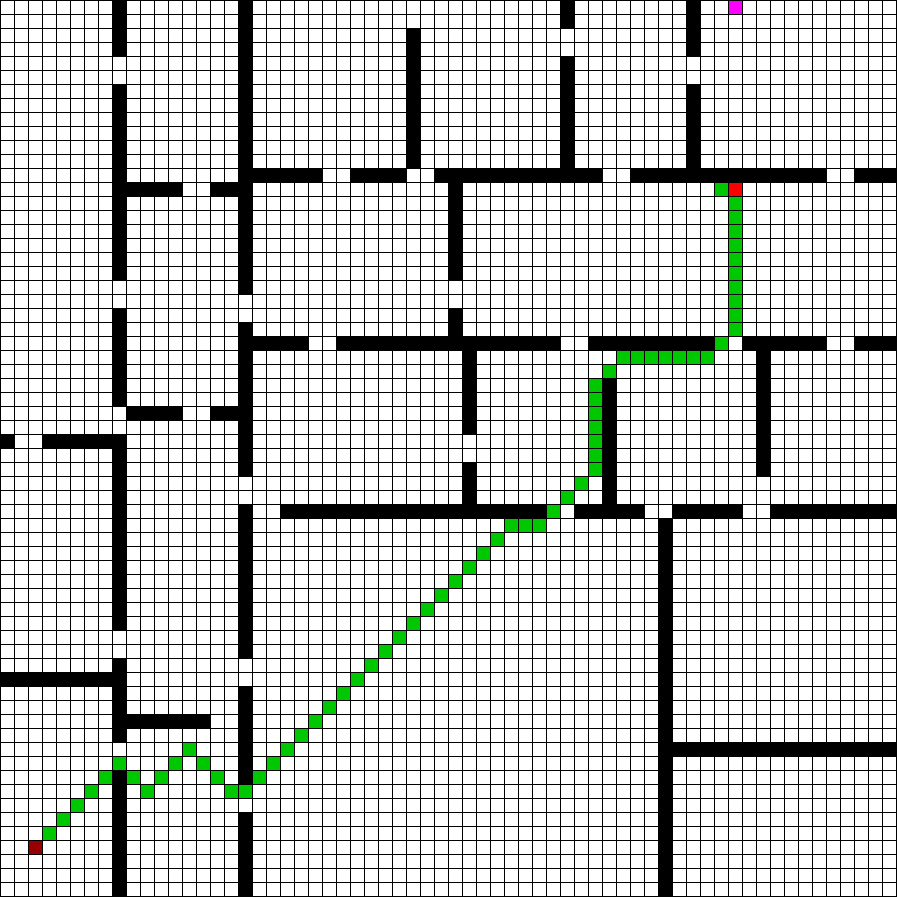
\includegraphics[width=\linewidth]{images/cae_lstm_4_block.png}
     \caption{CAE Online LSTM Planner}
  \end{subfigure}
  \caption{Online LSTM Planner vs CAE Online LSTM Planner}
  \label{fig: cae lstm vs lstm}
\end{figure}

\pagebreak

\section{LSTM Bagging Planner}

We currently have two solutions: Online LSTM Planner and CAE Online LSTM Planner. Both algorithms behave differently depending on the map layout. Moreover, we can notice the same behaviour variability when training the models on uncorrelated datasets. Thus, we introduce the LSTM Bagging Planner, which combines the performance of multiple models and picks the best behaving model depending on the map layout.

The idea was inspired by Ensemble Machine Learning methods \cite{dietterich2000ensemble}. Ensemble ML methods use multiple weak learners (other weak ML models such as Decision Stumps or Decision Trees) and, based on a majority voting consensus, outputs the classification choice. Ensemble ML is split into two categories: sequential and parallel. Sequential ensemble ML (e.g. AdaBoost) trains the weak learners sequentially on the same dataset. However, in order to make the learners independent of each other, the dataset is weighted. After training the first weak learner, if an example was wrongly classified, the weight associated with that particular sample will be increased (boosted) so that the next weak learner will classify the sample correctly (if an example was classified correctly, the weight is decreased). We are going to focus on the parallel ensemble methods which train all weak learners at the same time in parallel, but on different training datasets sampled from the original dataset. Thus, the weak learners are not correlated, and each one of them learns different features. Lastly, by having multiple uncorrelated weak learners, the voting procedure increases the accuracy of the predictions.

In our case, we use the Online LSTM and CAE Online LSTM Planners as our weak learners. Because the models can be trained on different generated training datasets (uniform random fill map, block map, house map) each weak learner learns how to behave in different environments (by extracting different features) and are uncorrelated.

The algorithm takes as input two arguments: $kernel\_names$ and $max\_it$. $kernel\_names$ defines the names of the weak learners (the name is based on the model type and training dataset). $max\_it$ is used to initialise all weak learners ((CAE) Online LSTM Planner takes $max\_it$ as input) and has the same effect as the $max\_it$ from the (CAE) Online LSTM Planner. Weak learners (kernels) are loaded and executed in parallel on the map. If any/multiple kernels have found the goal we pick the one which has lower traversed length. Otherwise, we pick the kernel which has made the furthest progress (longest traversed length). If at any point we have multiple kernels that satisfy the best kernel conditions, we pick the one that occurs first in $kernel\_names$ (i.e. higher priority is given to the first kernels). Lastly, we follow the best kernel path (See Algorithm \ref{alg: lstm bagging}).

\begin{algorithm}[]
\caption{LSTM Bagging Planner}
\label{alg: lstm bagging}
\begin{algorithmic}[1]
\Procedure{LSTM-Bagging-Planner}{$M\colon(A, Os, G)$, $kernel\_names$, $max\_it=\infty$}
    \State $kernels \gets$ load all $kernel\_names$ with maximum iterations $max\_it$
    \State $results \gets$ run all $kernels$ in parallel on $M$
    \State $best\_results \gets$ []
    \State
    \For{$result$ in $results$}
        \If{$result$ has reached $G$}
            \State append $result$ to $best\_results$
        \EndIf
    \EndFor
    \State
    \State $best\_result \gets \exists r1,\forall r2 \in best\_results. r1$ traversed length
    $\leq r2$ traversed length
    \State
    \If{$best\_result$ exists}
        \State execute $best\_result$ trace
        \State \Return
    \EndIf
    \State
    \State $best\_result \gets \exists r1,\forall r2 \in best\_results. r1$ traversed length
    $\geq r2$ traversed length
    \State
    \State execute $best\_result$ trace
\EndProcedure
\end{algorithmic}
\end{algorithm}

\pagebreak

\subsection{Complexity Analysis}

\begin{Theo}{2-dimensional Complexity}{3_2d_complex}
Worst case time complexity (2D environments; See \Cref{Th:3_1_2d_complex_general} for proof)):

\begin{align*}
    \mathcal{O}(LSTMBagging) = \mathcal{O}(xo + nm \log nm + \min(max\_it, d))
\end{align*}


%\begin{align*}
%    \mathcal{O}(LSTMBagging) = %\mathcal{O}(kernel\_number \, %(\mathcal{O}(OnlineLSTM) + %\mathcal{O}(CAEOnlineLSTM)))
%\end{align*}

Worst case space complexity (2D environments; See \Cref{Th:3_2_2d_complex_general} for proof)):

\begin{align*}
    \mathcal{O}(LSTMBagging) = \mathcal{O}(kernel\_number).
\end{align*}

where $xo$ is the inflation pre-process from \textbf{DenseMap} (this is also present in A* when it is run on a \textbf{DenseMap}), $x$ is the inflation rate, $o$ is the average obstacle size, $d$ is the solution depth and $n$, $m$ are the global image snapshot dimensions.

\end{Theo}

\begin{Theo}{General 2-dimensional Worst Case Time Complexity}{3_1_2d_complex_general}
The general worst case time complexity (2D environments) is:

\begin{align*}
    \mathcal{O}(LSTMBagging) = \mathcal{O}(kernel\_number \, (\mathcal{O}(OnlineLSTM) + \\ \mathcal{O}(CAEOnlineLSTM)))
\end{align*}

\begin{Proof}{}{test}

Because we run the kernels in parallel, the worst case time complexity becomes:

\begin{align*}
    \mathcal{O}(LSTMBagging) &= \mathcal{O}(\mathcal{O}(OnlineLSTM) + \mathcal{O}(CAEOnlineLSTM)) \\ &= \mathcal{O}(CAEOnlineLSTM) \\ &= \mathcal{O}(xo + nm \log nm + \min(max\_it, d))
\end{align*}

\end{Proof}

\end{Theo}

\begin{Theo}{General 2-dimensional Worst Case Space Complexity}{3_2_2d_complex_general}
The general worst case space complexity (2D environments) is:

\begin{align*}
    \mathcal{O}(LSTMBagging) = \mathcal{O}(kernel\_number \, (\mathcal{O}(OnlineLSTM) +\\ \mathcal{O}(CAEOnlineLSTM)))
\end{align*}

\begin{Proof}{}{test}
$\mathcal{O}(\mathcal{O}(OnlineLSTM) + \mathcal{O}(CAEOnlineLSTM)) = \mathcal{O}(1)$. 
\\

Thus, the worst case space complexity becomes: 
\begin{align*}
    \mathcal{O}(LSTMBagging) = \mathcal{O}(kernel\_number).
\end{align*}

It should be noted that, in the actual implementation we clone the map $kernel\_number$ times and feed each clone to the associated kernel, but this is due to the design of the simulator and it can easily be changed to use the same initial map.
\end{Proof}
\end{Theo}

\subsection{General Discussion}

The algorithm inherits all properties from the Online LSTM Planner and CAE Online LSTM Planner. Therefore, the optimal path is relatively close to the A* performance, and it is even improved as we pick the shortest suggested path (if one is found).

The advantage of using this method is that the success rate of finding the goal is significantly increased compared to the Online LSTM and CAE Online LSTM Planners due to the reasons mentioned above (i.e. weak learners are uncorrelated). Moreover, it shares the same time complexity as a single kernel (See Figure \ref{fig: LSTM Bagging Planner runs}) while inheriting the properties of all kernels.

The disadvantage is that, in practice, even if we run the kernels in parallel, there is a heavier resource load and the algorithm is usually slower than a single kernel. Lastly, there has been an implementation problem with \textit{python} threads. \textit{python} threads work differently than threads from other programming languages and usually do not improve the performance if the tasks are not interrupt driven (e.g. I/O tasks). Therefore, we have tried to replace threads with processes, but we could not do it as there was an issue when passing the data through the \textit{pytroch} modules. The issue has not been fixed, and we are running the kernels sequentially, but it should be noted that switching to a parallel architecture is plausible (\textit{pytroch} states that it supports multi-threading).

\begin{figure}[h!]
  \centerfloat
  \begin{subfigure}[b]{0.33\linewidth}
    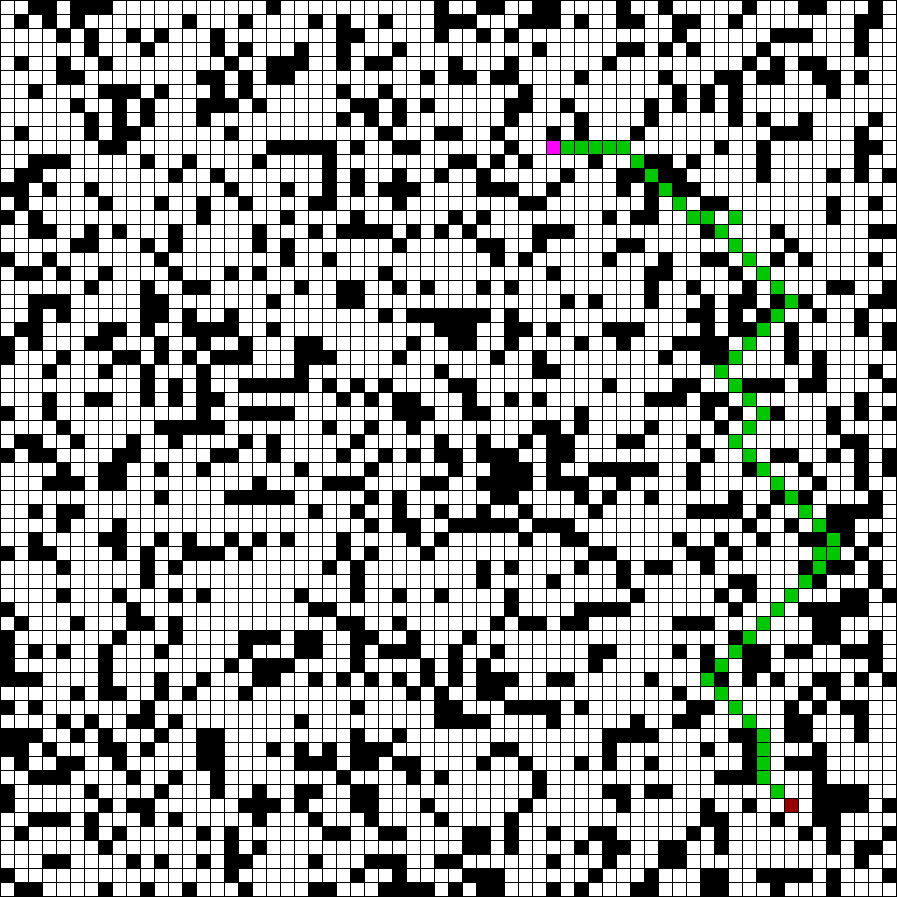
\includegraphics[width=\linewidth]{images/lstm_bagging_1.png}
     \caption{Goal found. Best kernel: CAE Online LSTM (\texttt{house\_10000})\newline \newline \newline}
  \end{subfigure}
  \hfill
  \begin{subfigure}[b]{0.33\linewidth}
    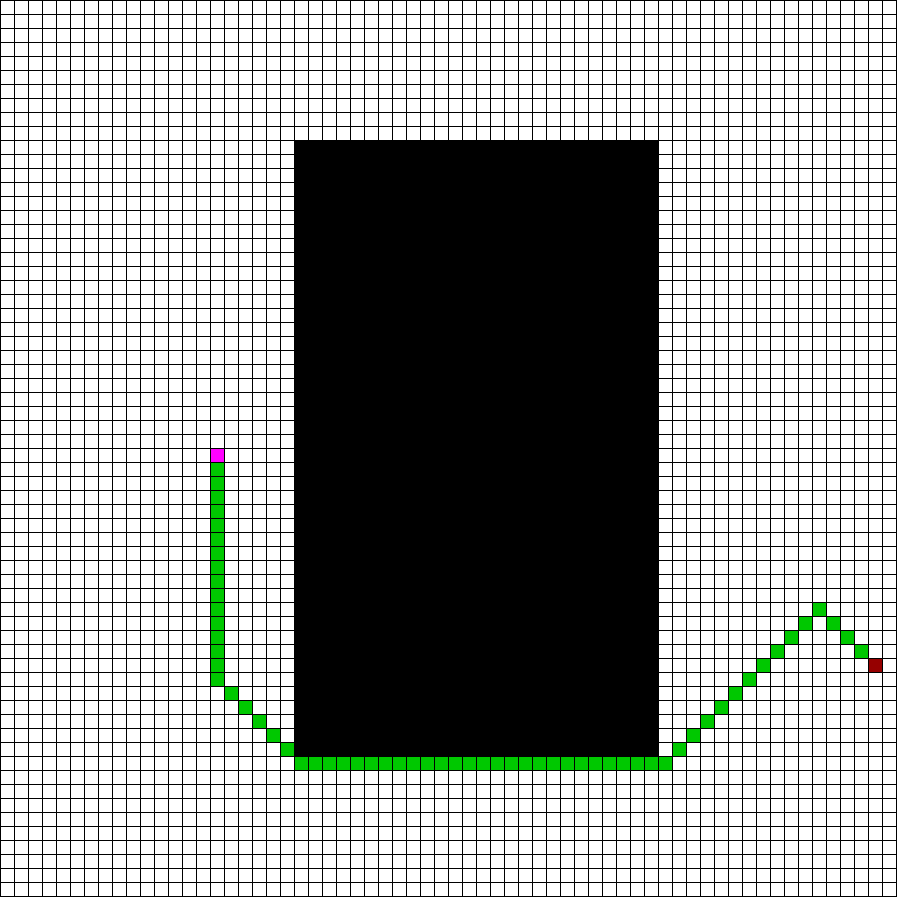
\includegraphics[width=\linewidth]{images/lstm_bagging_2.png}
     \caption{Path is shorter. Best kernel: CAE Online LSTM (\texttt{uniform\_random\_fill\_10000}, \texttt{block\_map\_10000}, \texttt{house\_10000})\newline}
  \end{subfigure}
  \hfill
  \begin{subfigure}[b]{0.33\linewidth}
    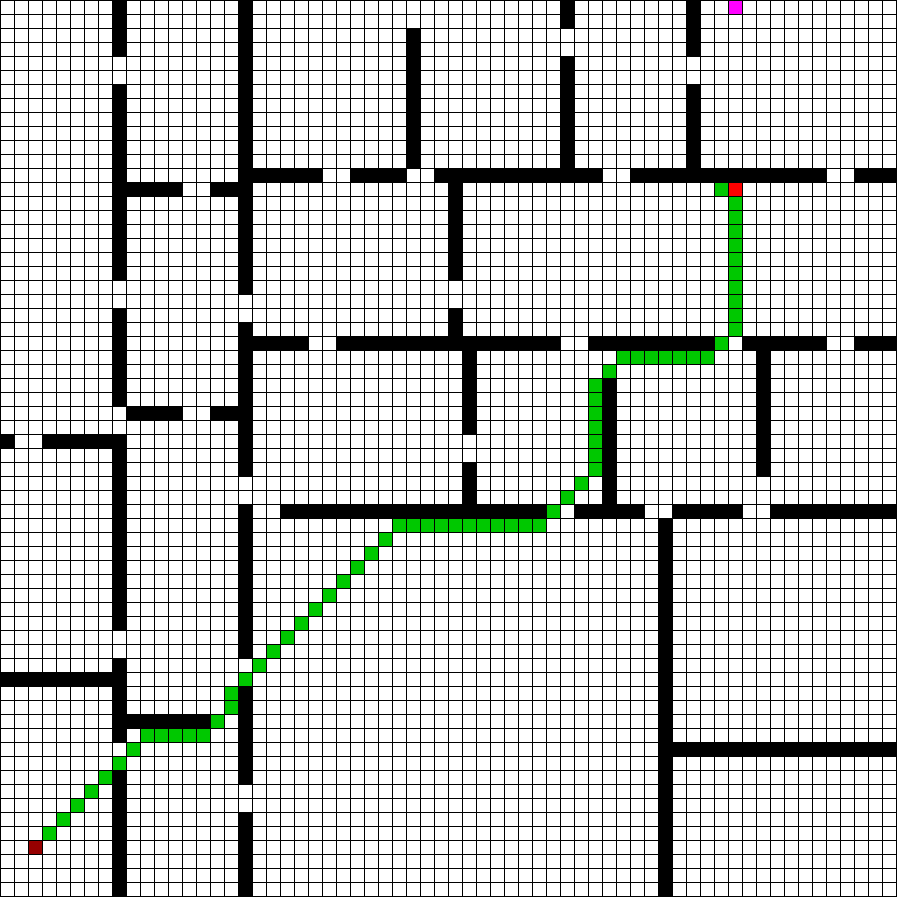
\includegraphics[width=\linewidth]{images/lstm_bagging_3.png}
     \caption{Goal not found, but is close to the goal. Best kernel: CAE Online LSTM (\texttt{uniform\_random\_fill\_10000}, \texttt{block\_map\_10000)}}
  \end{subfigure}
  \caption{LSTM Bagging Planner with 10 kernels (kernel configuration is described in Table \ref{tab:LSTM Bagging Planner config}) paths. The maps are identical to the ones used in the failed Online LSTM Planner runs (See figure \ref{fig: lstm path fail}). The parenthesis value represents the training dataset on which the planner was trained on}
  \label{fig: LSTM Bagging Planner runs}
\end{figure}

\begin{table}[h!]
    \centering
    \begin{tabular}{|c|c|}
         \hline
         \textbf{Kernel} & \textbf{Training Data} \\
         \hline
         \hline
         CAE Online LSTM & \texttt{block\_map\_10000} \\
         \hline
         CAE Online LSTM & \texttt{uniform\_random\_fill\_10000} \\
         \hline
         CAE Online LSTM & \texttt{house\_10000} \\
         \hline
         CAE Online LSTM & \texttt{uniform\_random\_fill\_10000\_block\_map\_10000\_house\_10000} \\
         \hline
         CAE Online LSTM & \texttt{uniform\_random\_fill\_10000\_block\_map\_10000} \\
         \hline
         \hline
         Online LSTM & \texttt{uniform\_random\_fill\_10000} \\
         \hline
         Online LSTM & \texttt{block\_map\_10000} \\
         \hline
         Online LSTM & \texttt{house\_10000} \\
         \hline
         Online LSTM & \texttt{uniform\_random\_fill\_10000\_block\_map\_10000} \\
         \hline
         Online LSTM & \texttt{uniform\_random\_fill\_10000\_block\_map\_10000\_house\_10000} \\
         \hline
    \end{tabular}
    \caption{LSTM Bagging Planner kernel configuration in priority order}
    \label{tab:LSTM Bagging Planner config}
\end{table}

\pagebreak

\section{Global Way-point LSTM Planner} \label{sec: way point nav}
% move statistics at the end
% move statistics to evaluation
% describe loss
After running empirical evaluations, we have noticed that the algorithms from previous sections get lost when the sequence size is too large. In order to overcome this issue, we introduce the Global Way-point LSTM Planner.

The Global Way-point LSTM Planner is a solution which makes use of two types of algorithms (kernels): local and global. The global kernel is responsible for producing a series of suggested global way-points and the local kernel is responsible for planning the trajectory between the way-points. For our scope, we are going to use one of the previous ML solutions (Online LSTM Planner, CAE Online LSTM Planner or LSTM Bagging Planner) as the global kernel. We can use any existing path planning solution for the local kernel, but we are going to use A* as it represents the main comparison frame of reference in Chapter \ref {Evaluation} (\hyperref[Evaluation]{Evaluation}).

The algorithm accepts three inputs: the $local\_kernel$, $global\_kernel$ and $gk\_max\_it$. $gk\_max\_it$ is used to initialise the $global\_kernel$ and is correlated with the distance between way-points. At each iteration, the $local\_kernel$ and $global\_kernel$ are reset. If the last way-point is not the goal itself, the local kernel is run one more time from the last way-point to the goal. As in the Online LSTM planner, we have included a fail-safe mechanism which breaks the main loop if a location is visited more than 5 times (See Algorithm \ref{alg: way-point}).

\begin{algorithm}[]
\caption{Global Way-point LSTM Planner}
\label{alg: way-point}
\begin{algorithmic}[1]
\Procedure{Global-Way-point-LSTM-Planner}{$M\colon(A, Os, G)$, $local\_kernel$, $global\_kernel$, $gk\_max\_it$}
    \State
    \State Initialise $local\_kernel$
    \State Initialise $global\_kernel$ with $gk\_max\_it$
    \State $history\_frequency \gets \{\colon\}$
    \State
    \While{True}
        \State $trace \gets$ execute $global\_kernel$
        \State $way\_point \gets$ last $trace$ position
        \State $trace \gets$ execute $local\_kernel$ from $A$ to $way\_point$
        \State follow $trace$
        \State
        \State $history\_frequency[A] \gets 1$ (if no value) or $history\_frequency[A] + 1$
        \State
        \If {$history\_frequency[A] > 5$}
            \State \textbf{break}
        \EndIf
        \State
        \If {goal was reached}
            \State \textbf{break}
        \EndIf
    \EndWhile
    \State
    \If {goal was not reached}
        \State $trace \gets$ execute $local\_kernel$
        \State follow $trace$
    \EndIf
\EndProcedure
\end{algorithmic}
\end{algorithm}

\subsection{Complexity Analysis}

\begin{Theo}{2-dimensional Worst Case Complexity}{4_2d_complex}
The worst case time and space complexities (2D environments) are inherited from the local and global kernel:

\begin{align*}
    \mathcal{O}(GlobalWaypointLSTM) = \mathcal{O}(\mathcal{O}(local\_kernel) + \mathcal{O}(global\_kernel))
\end{align*}

It should be noted that the map is cloned when passed over to the kernels, but this is due to the simulator design and can easily be switched to passing a reference to the map instead.
\end{Theo}

\begin{Theo}{2-dimensional Average Case Complexity}{4_2d_complex_average}
The average case time and space complexity (2D environments) is: 

\begin{align*}
    \mathcal{O}(GlobalWaypointLSTM) = \mathcal{O}(\frac{gk\_max\_it}{d}\,(\mathcal{O}(local\_kernel) + \mathcal{O}(global\_kernel)))
\end{align*}

where $d$ is the solution depth. 
\\

The complexity is equivalent to the average session complexity of the local and global kernel.
\end{Theo}

\subsection{General Discussion}

The major advantage of using this method is that we can transform the Online LSTM, CAE Online LSTM or LSTM Bagging Planners into way-point suggestion algorithms and thus, the sequence size is reduced, and the performance is improved. Moreover, we can use A* as our local kernel to ensure that we always find a path if we fail to place the last way-point on the goal. The local kernel can even be switched with a randomized kinodynamic solution (a planning solution which takes into account vehicle constraints such as velocity and torque) such as RRT. Because we use online global kernel solutions, we support partial information environments as the map can be queried again when we reach a new way-point. In order to support dynamic environments, we can switch the local kernel with an online planner that supports dynamic environments (we can even use Online LSTM, CAE Online LSTM or LSTM Bagging Planners themselves). Furthermore, the worst case time and space complexity of the algorithm is equal to A*: $\mathcal{O}(GlobalWaypointLSTM) = \mathcal{O}(\mathcal{O}(local\_kernel) + \mathcal{O}(global\_kernel)) = \mathcal{O}(\mathcal{O}(A*) + \mathcal{O}(global\_kernel)) = \mathcal{O}(A*)$. Lastly, the average time and space complexity is less than or equal to A*: $\mathcal{O}(GlobalWaypointLSTM) = \mathcal{O}(\frac{gk\_max\_it}{d}\,(\mathcal{O}(local\_kernel) + \mathcal{O}(global\_kernel))) = \mathcal{O}(\frac{gk\_max\_it}{d}\,(\mathcal{O}(A*) + \mathcal{O}(global\_kernel))) \leq \mathcal{O}(A*)$ (if the way-points are well distributed the performance is improved quite a lot) (See Figure \ref{fig: Way runs} and Figure \ref{fig: Way runs comp}).

The major disadvantage to this approach is that the algorithm does not usually find the optimal path if the global kernel does not suggest optimal way-points, but because we are using the Online LSTM, CAE Online LSTM or LSTM Bagging Planners as the global kernel we receive a close to optimal path. Nonetheless, if we are using the A* local kernel, we have an optimal path between way-points.

\pagebreak

\begin{figure}[h!]
  \centerfloat
  \begin{subfigure}[b]{0.33\linewidth}
    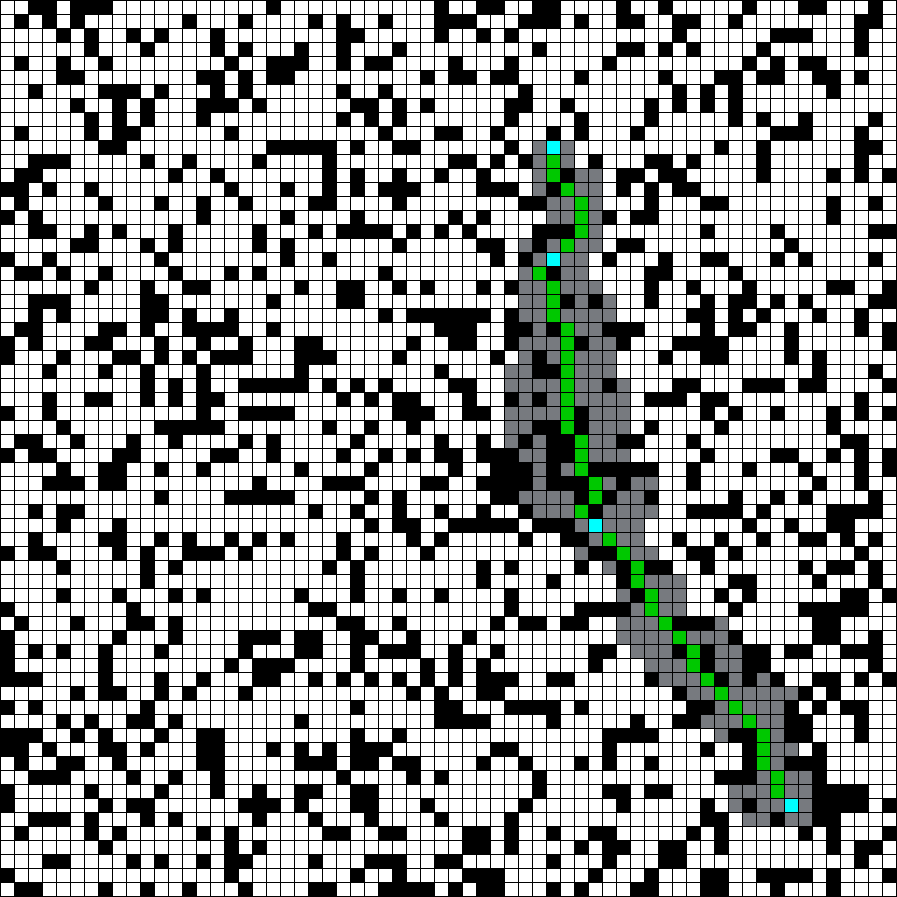
\includegraphics[width=\linewidth]{images/way-point_nav_1.png}
     \caption{Goal found. Distance: 57.36 \newline} %Pick Ratio: [0.0\%, 66.67\%, 0.0\%, 0.0\%, 0.0\%, 0.0\%, 0.0\%, 33.33\%, 0.0\%, 0.0\%]}
  \end{subfigure}
  \hfill
  \begin{subfigure}[b]{0.33\linewidth}
    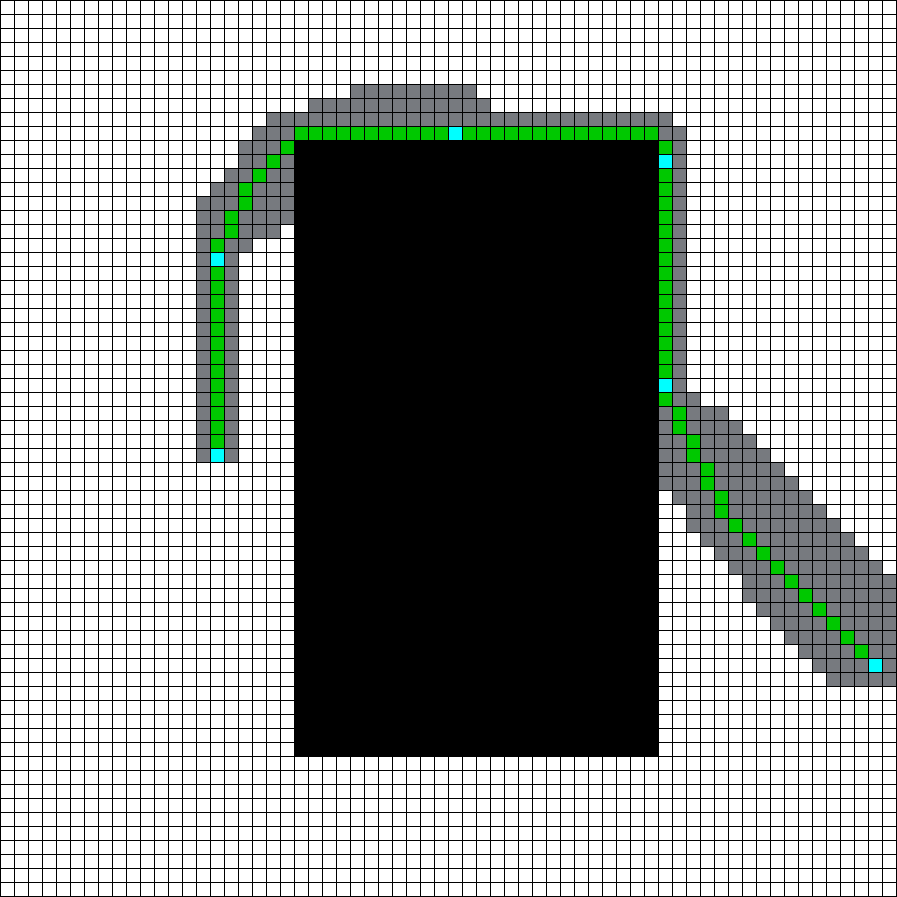
\includegraphics[width=\linewidth]{images/way-point_nav_2.png}
     \caption{Path is insignificantly shorter. Distance: 95.11} % Pick Ratio: [100.0\%, 0.0\%, 0.0\%, 0.0\%, 0.0\%, 0.0\%, 0.0\%, 0.0\%, 0.0\%, 0.0\%]}
  \end{subfigure}
  \hfill
  \begin{subfigure}[b]{0.33\linewidth}
    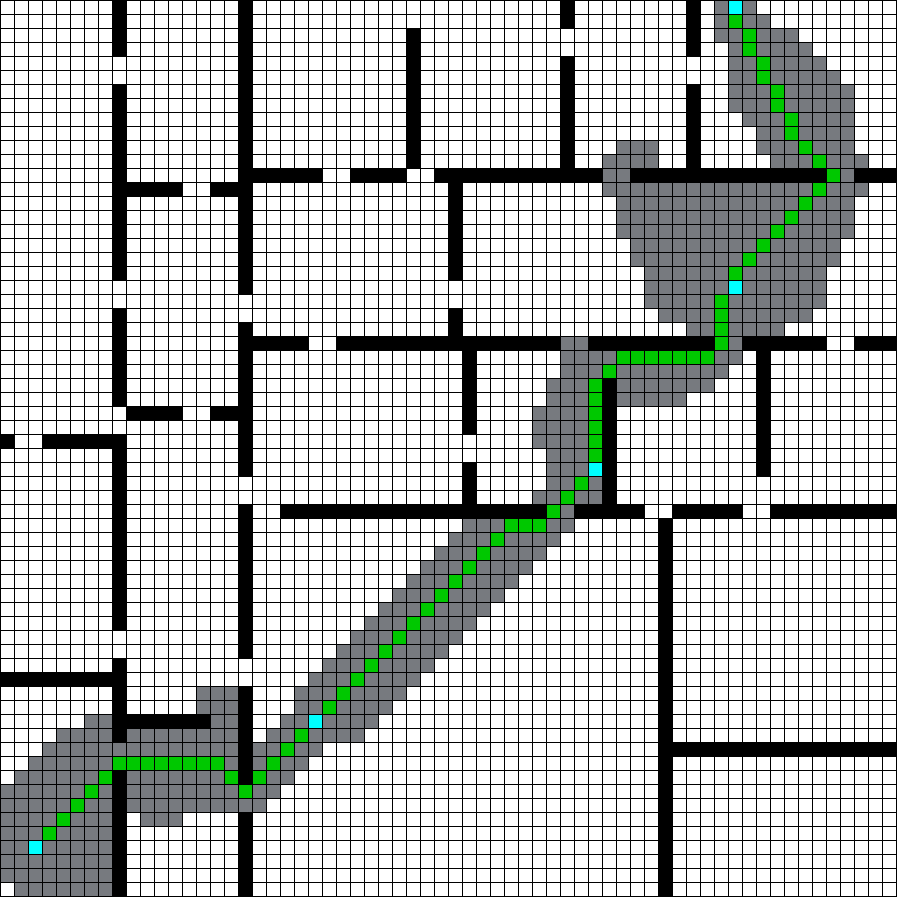
\includegraphics[width=\linewidth]{images/way-point_nav_3.png}
     \caption{Goal found. Distance: 99.30 \newline}% Pick Ratio: [75.0\%, 0.0\%, 25.0\%, 0.0\%, 0.0\%, 0.0\%, 0.0\%, 0.0\%, 0.0\%, 0.0\%]}
  \end{subfigure}
  \caption{Global Way-point LSTM Planner with local kernel A* and global kernel LSTM Bagging Planner (kernel configuration is described in Table \ref{tab:LSTM Bagging Planner config}). The maps are identical to the ones used in the failed Online LSTM runs (See figure \ref{fig: lstm path fail}). The produced path highly depends on the kernel priority. It should be noted that we display \textbf{all} memory used, but the average session memory is significantly smaller}
  \label{fig: Way runs}
\end{figure}

\begin{figure}[h!]
  \centerfloat
  \begin{subfigure}[b]{0.33\linewidth}
    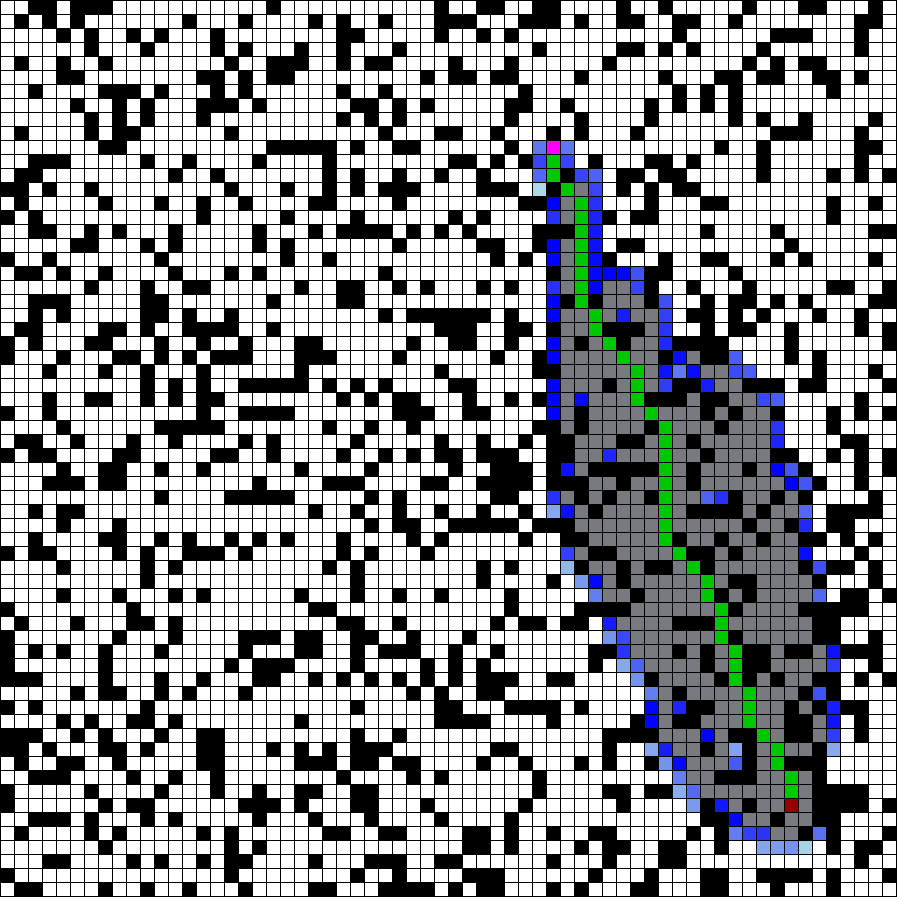
\includegraphics[width=\linewidth]{images/a_star_1_map.png}
    \caption{Path is a bit shorter. Distance: 54.04. A* memory uses more memory}
  \end{subfigure}
  \hfill
  \begin{subfigure}[b]{0.33\linewidth}
    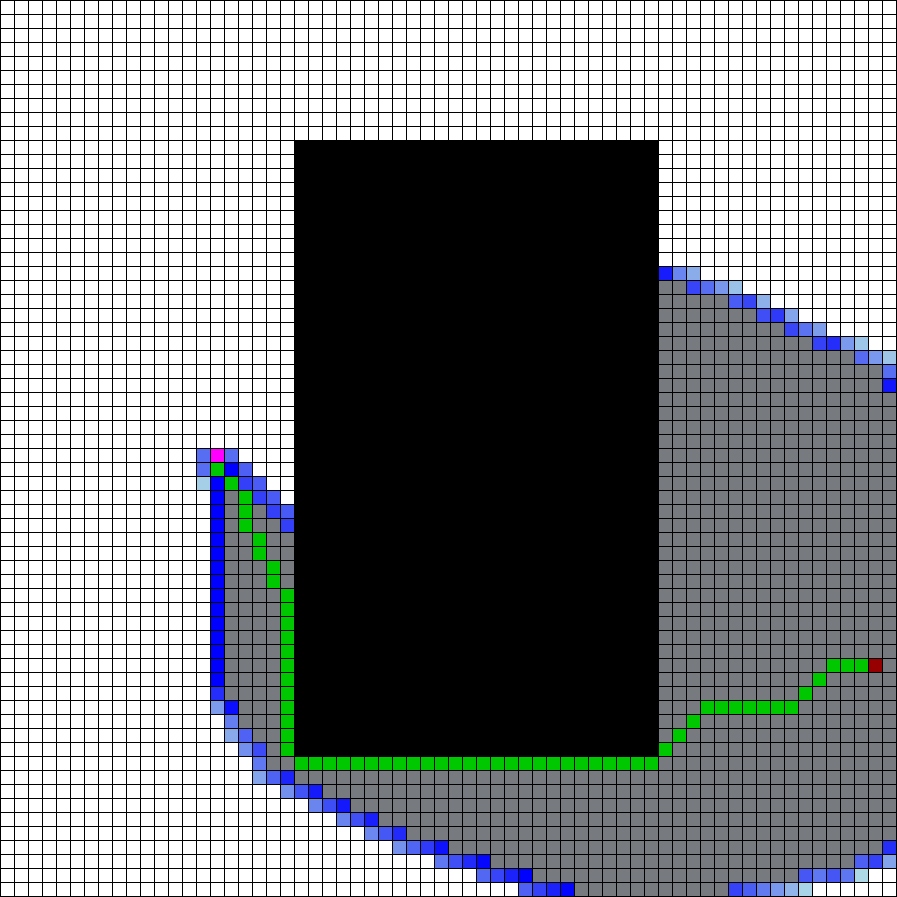
\includegraphics[width=\linewidth]{images/a_star_2_map.png}
    \caption{Path is shorter. Distance: 68.38. A* uses more memory \newline}
  \end{subfigure}
  \hfill
  \begin{subfigure}[b]{0.33\linewidth}
    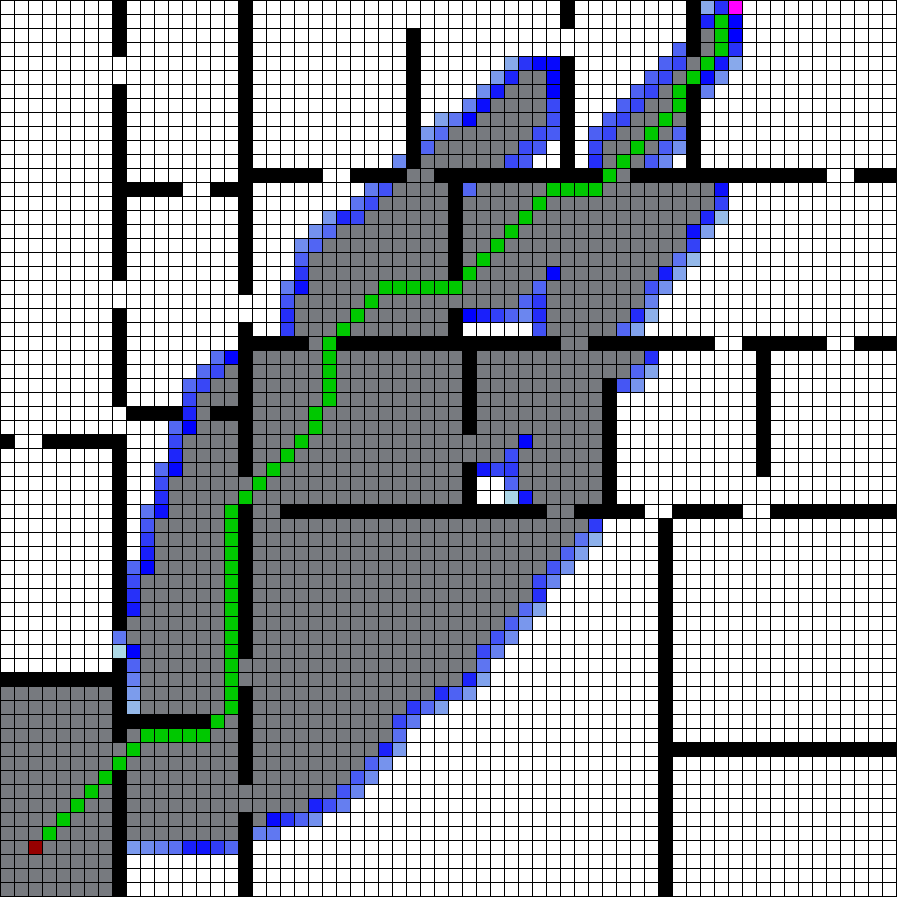
\includegraphics[width=\linewidth]{images/a_star_3_map.png}
    \caption{Path is a bit shorter. Distance: 87.74. A* uses more memory\newline}
  \end{subfigure}
  \caption{A* comparison to figure \ref{fig: Way runs}}
  \label{fig: Way runs comp}
\end{figure}

\pagebreak